\documentclass[floatsintext,doc]{apa6}

\usepackage{amssymb,amsmath}
\usepackage{ifxetex,ifluatex}
\usepackage{fixltx2e} % provides \textsubscript
\ifnum 0\ifxetex 1\fi\ifluatex 1\fi=0 % if pdftex
  \usepackage[T1]{fontenc}
  \usepackage[utf8]{inputenc}
\else % if luatex or xelatex
  \ifxetex
    \usepackage{mathspec}
    \usepackage{xltxtra,xunicode}
  \else
    \usepackage{fontspec}
  \fi
  \defaultfontfeatures{Mapping=tex-text,Scale=MatchLowercase}
  \newcommand{\euro}{€}
\fi
% use upquote if available, for straight quotes in verbatim environments
\IfFileExists{upquote.sty}{\usepackage{upquote}}{}
% use microtype if available
\IfFileExists{microtype.sty}{\usepackage{microtype}}{}

% Table formatting
\usepackage{longtable, booktabs}
\usepackage{lscape}
% \usepackage[counterclockwise]{rotating}   % Landscape page setup for large tables
\usepackage{multirow}		% Table styling
\usepackage{tabularx}		% Control Column width
\usepackage[flushleft]{threeparttable}	% Allows for three part tables with a specified notes section
\usepackage{threeparttablex}            % Lets threeparttable work with longtable

% Create new environments so endfloat can handle them
% \newenvironment{ltable}
%   {\begin{landscape}\begin{center}\begin{threeparttable}}
%   {\end{threeparttable}\end{center}\end{landscape}}

\newenvironment{lltable}
  {\begin{landscape}\begin{center}\begin{ThreePartTable}}
  {\end{ThreePartTable}\end{center}\end{landscape}}




% The following enables adjusting longtable caption width to table width
% Solution found at http://golatex.de/longtable-mit-caption-so-breit-wie-die-tabelle-t15767.html
\makeatletter
\newcommand\LastLTentrywidth{1em}
\newlength\longtablewidth
\setlength{\longtablewidth}{1in}
\newcommand\getlongtablewidth{%
 \begingroup
  \ifcsname LT@\roman{LT@tables}\endcsname
  \global\longtablewidth=0pt
  \renewcommand\LT@entry[2]{\global\advance\longtablewidth by ##2\relax\gdef\LastLTentrywidth{##2}}%
  \@nameuse{LT@\roman{LT@tables}}%
  \fi
\endgroup}


  \usepackage{graphicx}
  \makeatletter
  \def\maxwidth{\ifdim\Gin@nat@width>\linewidth\linewidth\else\Gin@nat@width\fi}
  \def\maxheight{\ifdim\Gin@nat@height>\textheight\textheight\else\Gin@nat@height\fi}
  \makeatother
  % Scale images if necessary, so that they will not overflow the page
  % margins by default, and it is still possible to overwrite the defaults
  % using explicit options in \includegraphics[width, height, ...]{}
  \setkeys{Gin}{width=\maxwidth,height=\maxheight,keepaspectratio}
\ifxetex
  \usepackage[setpagesize=false, % page size defined by xetex
              unicode=false, % unicode breaks when used with xetex
              xetex]{hyperref}
\else
  \usepackage[unicode=true]{hyperref}
\fi
\hypersetup{breaklinks=true,
            pdfauthor={},
            pdftitle={Generic statements have weak (and strong) implications},
            colorlinks=true,
            citecolor=blue,
            urlcolor=blue,
            linkcolor=black,
            pdfborder={0 0 0}}
\urlstyle{same}  % don't use monospace font for urls

\setlength{\parindent}{0pt}
%\setlength{\parskip}{0pt plus 0pt minus 0pt}

\setlength{\emergencystretch}{3em}  % prevent overfull lines


% Manuscript styling
\captionsetup{font=singlespacing,justification=justified}
\usepackage{csquotes}
\usepackage{upgreek}



\usepackage{tikz} % Variable definition to generate author note

% fix for \tightlist problem in pandoc 1.14
\providecommand{\tightlist}{%
  \setlength{\itemsep}{0pt}\setlength{\parskip}{0pt}}

% Essential manuscript parts
  \title{Generic statements have weak (and strong) implications}

  \shorttitle{Context-sensitive generic interpretations}


  \author{Michael Henry Tessler\textsuperscript{1}~\& Noah D. Goodman\textsuperscript{1}}

  % \def\affdep{{"", ""}}%
  % \def\affcity{{"", ""}}%

  \affiliation{
    \vspace{0.5cm}
          \textsuperscript{1} Department of Psychology, Stanford University  }

  \authornote{
    This manuscript is currently in prep. Comments or suggestions should be
    directed to MH Tessler.
    
    Correspondence concerning this article should be addressed to Michael
    Henry Tessler, 450 Serra Mall, Bldg. 420, Rm. 316, Stanford, CA 94305.
    E-mail:
    \href{mailto:mhtessler@stanford.edu}{\nolinkurl{mhtessler@stanford.edu}}
  }


  \abstract{Enter abstract here. Each new line herein must be indented, like this
line.}
  \keywords{keywords \\

    \indent Word count: X
  }




  \usepackage{tabularx}
  \usepackage{multicol}
  \usepackage{wrapfig}
  \usepackage{caption}
  \usepackage{booktabs}
  \usepackage{amsmath}
  \usepackage{graphicx}
  \usepackage{subcaption}
  \usepackage{longtable}
  \usepackage{array}
  \usepackage{multirow}

\usepackage{amsthm}
\newtheorem{theorem}{Theorem}
\newtheorem{lemma}{Lemma}
\newtheorem{corollary}{Corollary}
\newtheorem{proposition}{Proposition}
\newtheorem{conjecture}{Conjecture}
\theoremstyle{definition}
\newtheorem{definition}{Definition}
\theoremstyle{definition}
\newtheorem{example}{Example}
\theoremstyle{definition}
\newtheorem{exercise}{Exercise}
\theoremstyle{remark}
\newtheorem*{remark}{Remark}
\newtheorem*{solution}{Solution}
\begin{document}

\maketitle

\setcounter{secnumdepth}{0}



\newcommand{\denote}[1]{\mbox{ $[\![ #1 ]\!]$}}
\newcommand*\diff{\mathop{}\!\mathrm{d}}

\definecolor{Red}{RGB}{255,0,0} \definecolor{Green}{RGB}{10,200,100}
\definecolor{Blue}{RGB}{10,100,200}

\newcommand{\mht}[1]{{\textcolor{Blue}{[mht: #1]}}}
\newcommand{\ndg}[1]{{\textcolor{Green}{[ndg: #1]}}}
\newcommand{\red}[1]{{\textcolor{Red}{#1}}}







\section{Introduction}\label{introduction}

Learning from language is uniquely powerful because language can convey
information that is difficult or dangerous to observe (e.g., learning
that certain plants are poisonous, staring at the sun causes blindness;
Gelman, 2009). The premier example of language's ability to transmit
abstract knowledge comes in the form of statements that convey
generalizations, otherwise known as \emph{generic language} (e.g.,
``Birds fly''; Carlson, 1977). One of the most important roles for
generic language is to provide learners with information about new or
poorly understood categories. As such, generics are ubiquitous in
everyday conversation and child-directed speech (Gelman, Coley,
Rosengren, Hartman, \& Pappas, 1998; Gelman, Goetz, Sarnecka, \& Flukes,
2008; Gelman, Taylor, Nguyen, Leaper, \& Bigler, 2004), and learning
from generics is thought to be central to conceptual development
(Cimpian \& Markman, 2009; Gelman, 2004). Understanding how beliefs are
updated from generic language is thus an important question for cognitive
science.

Abelson and Kanouse (1966) argued that generics, \enquote{\ldots{}once
accepted psychologically, {[}\ldots{}{]} appear to be commonly taken in
a rather strong sense, as though the qualifier \emph{always} had
implicitly crept into their interpretation} (p.~172). Gelman, Star, and
Flukes (2002) provided adults with generics about animals with
non-obvious properties (e.g., \enquote{Bears like to eat ants}) and
found that the \emph{implied prevalence} of the feature among category
members (e.g., the percentage of bears that like to eat ants) was high
(\(\sim 85\%\)). Similarly strong interpretations were reported using
novel categories with biological properties (e.g., ``Lorches have purple
feathers''; Cimpian, Brandone, \& Gelman, 2010, Expt. 1). The fact that
generics seem to convey strong implications may explain why social stereotypes are propagated and maintained (Rhodes,
Leslie, \& Tworek, 2012).

Do all generics carry strong implications? \enquote{Mosquitos carry
malaria} really seems to only have the quantificational force of an
existential claim, meaning \emph{some mosquitos carry malaria}. This may
not be a unique example: Cohen (2004) argues for a panolply of
conditions that give rise to \emph{existential generics} (e.g.,
focus-sensitive additives, as in \enquote{Birds lay eggs. Mammals lay
eggs too.}: the second sentence can be interpreted as true because of
the existence of platypuses and echidnas, both of which reproduce by
laying eggs). Using a similar implied prevalence task as Gelman et al.
(2002), Cimpian et al. (2010) (Expt. 3) found somewhat weaker
interpretations for features that could be construed as accidental
(e.g., ``Crullets have fungus-covered claws''; see also Khemlani,
Leslie, \& Glucksberg, 2009, 2012 for evidence for weak inferences from
generics). 
In these
previous studies, the actual implied prevalence from \enquote{weak}
generics is still quite high (in Cimpian et al., 2010 Expt. 3, mean
implied prevalence \(= 70\%\)), leaving open the question of whether
generics can actually have weak interpretations (e.g., minority
interpretations: \(< 50\%\)).
There are also open theoretical questions:
property-specific generic interpretations have been explained as
theory-based expectations (Cimpian, Gelman, \& Brandone, 2010; Leslie,
2008; Prasada, Khemlani, Leslie, \& Glucksberg, 2013), but these notions
have not been made sufficiently precise to provide a quantitive,
predictive account of how beliefs will be updated given a specific generic statement. 

Tessler and Goodman (under review) proposed a quantitative model of
generic language, which combines tools from formal semantics and Bayesian modeling. 
This model accounted for truth judgments or endorsements (e.g., is
\enquote{Mosquitos cary malaria} true or false?) about a wide range of
linguistic stimuli including generics about animals, habitual statements
about actions (e.g., \enquote{John runs}), and causal language (e.g.,
\enquote{This herb makes animals sleepy}). This endorsement model is
cast as a speaker deciding whether or not to assert a generic statement to
a listener, who will update her beliefs from the generic
statement. The listener model used therein provides a mapping from a
generic statement to implied prevalence---it is a quantitative account
of how generics update beliefs. This paper tests the predictions of this listener
model directly. In doing so, we also look for evidence for \emph{weak generics},
which are predicted by the model and provide the strongest test of our unified quantitative account.

The paper is organized as follows. First, we review Tessler and Goodman
(under review)'s computational model of generic interpretation. In Expt.
1, we replicate and extend the findings of Cimpian et al. (2010) that
biological and accidental properties receive differential
interpretations. In Expt. 2, we extend these findings using a larger and
more diverse stimulus set better able to test the quantitative
predictions of our model and explore the existence of \enquote{weak
generics}. In Expt. 3, we experimentally manipulate the background
knowledge (the feature prevalence prior distirbution) and test its effect on interpretations
of novel generics. In each experiment, we compare our model's
predictions to alternative models, \ndg{say briefly what the alternative models are} finding that our quantitative model
is best able to account for generic interpretations across conditions.
Together, these results provide strong evidence for a quantitative
understanding of generic language. \ndg{that last sentence sounds somewhat vacuous... rephrase to be more contentfull?}

\section{Computational model}\label{computational-model}

Generic language conveys generalizations about categories (Carlson,
1977; Leslie, 2008). Probability is a useful representation for human
generalization from observational data (Shepard, 1987; Tenenbaum, Kemp,
Griffiths, \& Goodman, 2011), and so it makes sense that probability
would be at the core of the meaning of generalizations conveyed in language.
Tessler and Goodman (under review) formalize such a hypothesis, positing
that the semantics of generics has to do with probability but in an
underspecified or vague way.

Using the truth-functional tools of formal semantics (Montague, 1973),
the literal meaning of a generic statement can be modeled as a threshold
function operating on the prevalence \(r\) of the feature in the
category (e.g., the proportion of mosquitos that carry malaria) \ndg{might want to add the footnote that r doesn't have to be empirical frequency, but can be taken to be subjective probability?}:
\(\denote{generic} = \{r > \theta\}\). The literal meaning of
quantifiers can also be described by a threshold-function (e.g.,
\(\denote{some} = \{r > 0\}\), \(\denote{most} = \{r > 0.5\}\),
\(\denote{all} = \{r = 1\}\)). Tessler and Goodman (under review) posit
that the corresponding threshold for the generic \(\theta\) is \emph{a
priori} uncertain---formally, is drawn from a context-invariant, uniform
prior distribution on thresholds \(P(\theta)\)---and is resolved by
context.

In order for a statement to update beliefs about prevalence in a given category, a listener
must have prior beliefs about prevalence across categories. To interpret a generic
sentence, a listener draws upon abstract knowledge about properties,
formalized by a prior distribution over likely prevalence levels
\(P(r)\).\footnote{Though not the direct focus of this work, the
  prevalence prior distribution can be seen as a relatively shallow
  formalization of theory-based expectations. Different theory-based
  relationships between kinds and properties will give rise to different
  prior distributions over prevalence. The prevalence prior, thus, acts
  as a statistical layer between conceptual knowledge and natural
  language semantics.} Thus the quantitative model for generic
interpretation is given by:

\begin{eqnarray}
L(r, \theta \mid u) &\propto& {\delta_{\denote{u}(r, \theta)} \cdot P(r) \cdot P(\theta)} \label{eq:L0}
\end{eqnarray}

Formally, the truth-functional meaning is represented by the Kronecker
delta function \(\delta_{\denote{u}(r, \theta)}\) that returns
\(1\) when the utterance is true (i.e.,
when \(r > \theta\)) and \(0\) otherwise.

\begin{eqnarray}
\delta_{\denote{u_{gen}}(r, \theta)} &\propto  & \begin{cases}
1 & \text{if } r > \theta \\
0 & \text{otherwise}
\end{cases}\label{eq:delta}
\end{eqnarray}

The interpretation model computes a posterior distribution on prevalence
by considering different possible thresholds \(\theta\). Given a
particular value of \(\theta\), the literal semantics rules out all
prevalences \(r\) below \(\theta\). With a uniform prior over prevalence
(\(P(r) = \text{Uniform}(0, 1)\)), the posterior on prevalence will be
uniform over all prevalence levels above \(\theta\)
(Figure~\ref{fig:modelSimulations}B; top row). Because higher prevalence
levels are consistent with more thresholds, the generic interpretation
model returns a non-uniform posterior that favors higher prevalence
levels (Figure~\ref{fig:modelSimulations}B; top row, right-most column).
This behavior is consistent with the intuition that, without strong
background knowledge, generics imply that most or all of the category
has the property.

In this model, different interpretations come from different prior
distributions over prevalence \(P(r)\). The prevalence prior for a
purely abstract property may be given by a uniform distribution, while
prevalence priors for familiar properties may display interesting
structure reflecting domain-specific beliefs about the property.
Figure~\ref{fig:modelSimulations}A shows hypothetical prevalence priors
for the features \emph{fly} and \emph{carry malaria} as well as an
abstract property \emph{Y} without structured background knowledge. The
distribution over a biological property like \emph{fly} (which would
be used in interpreting generics like \enquote{Ducks fly}) is bimodal
with modes near 0\% and 100\%, reflecting the idea that for an arbitrary
category, it is likely that 0\% of them fly (e.g., dogs, rabbits,
etc\ldots{}); however, among categories with at least some members who
fly, we would expect all or nearly all of them to fly (hence, the second
mode near 100\%). The distribution over prevalence for a somewhat
accidental property like \emph{carry malaria} (as in \enquote{Mosquitos
carry malaria}) also has substantial probability mass at or near 0\%,
since most categories do not have the property present at all. However,
among categories with at least a few members who carry malaria, it is
very unlikely that all or even many carry malaria; the second mode of
this distribution is near 10\%. In this way, the prevalence prior can be
viewed as a distribution over different categories (and their associated
prevalence of the feature).

The generic interpretation model balances the prior probability of
different prevalence levels with the overall preference for higher
prevalence levels (as described above), producing interpretations that
appear similar to different quantified statements depending on the
property in question (Figure~\ref{fig:modelSimulations}B). For the biological
property prior, \enquote{Xs fly} is interpreted most similarly to
\enquote{Most Xs fly} and not \enquote{Some Xs fly}. For the accidental
property prior, \enquote{Xs carry malaria} is more similar to
\enquote{Some Xs carry malaria} than \enquote{Most Xs carry malaria}. We
test these property-sensitive interpretations in the following
experiments.

\ndg{note: i changed "context" to other things (eg "property") in a bunch of places because what we're talking about is differences in target property and it's corresponding background knowledge. this is context in some sense, but i worry it would confuse people with more pragmatic / situated notions of context.}

\begin{figure}
\centering
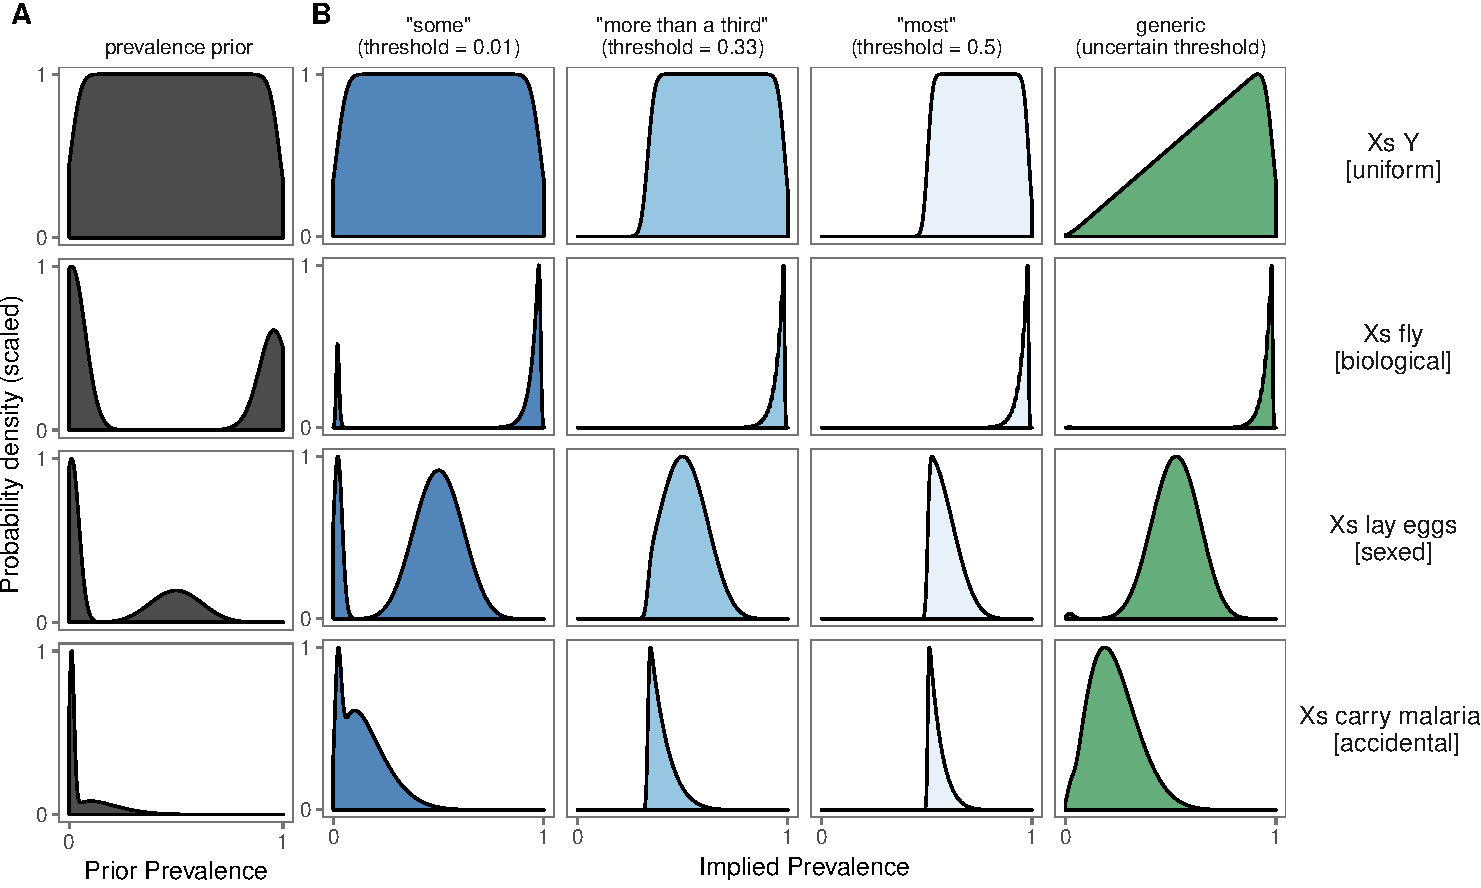
\includegraphics{genint_files/figure-latex/modelSimulations-1.pdf}
\caption{\label{fig:modelSimulations}Model simulations. A: Prevalence priors
reflect knowledge about properties. An abstract property could be given
a uniform distribution, while familiar properties display more complex
structure. B: Posterior distributions over prevalence (interpretations)
given different fixed-threshold quantifiers and the uncertain threshold
generic.}
\end{figure}

\section{Experiment 1: Replication and extension of Cimpian et al.
(2010)}\label{experiment-1-replication-and-extension-of-cimpian-et-al.-2010}

Our model of generic interpretation (Eq. \ref{eq:L0}) predicts that the
interpretations of generics in terms of prevalence should vary as a
function of the prevalence prior. Cimpian et al. (2010) found a
difference in the implied prevalence between biological properties
(e.g., \emph{yellow fur}) and accidental properties (e.g.,
\emph{fungus-covered claws}). Classic work in generalization suggests
beliefs about the prevalence of properties include relatively fine
distinctions among properties that are all biological in nature
(Nisbett, Krantz, Jepson, \& Kunda, 1983). For this reason, we
elaborated the stimulus set from Cimpian et al. (2010) to include three
types of biological properties: body parts (e.g., \emph{fur}), body
parts of a particular color (e.g., \emph{yellow fur}) and body parts
described with a vague adjective (e.g., \emph{curly fur}). Here, we
empirically measure the prevalence priors for these properties using a structured prior
elicitation task (Expt. 1a) and use our interpretation model to predict
the prevalence implied by a generic statement about a novel category
(e.g., \enquote{Wugs have yellow fur}; Expt. 1b).

\subsection{Experiment 1a: Prior
elicitation}\label{experiment-1a-prior-elicitation}

This experiment measures the prevalence prior \(P(r)\) in Eq.
\ref{eq:L0} using a structured, prior elicitation procedure.

\subsubsection{Method}\label{method}

\paragraph{Participants}\label{participants}

We recruited 40 participants over Amazon's crowd-sourcing platform
Mechanical Turk (MTurk). We chose this number of participants based on
intuition from similar experiments which were designed primarily to test
a quantitative model. Participants were restricted to those with US IP
addresses and with at least a 95\% MTurk work approval rating. All
participants were native English speakers. The experiment took about 5-7
minutes and participants were compensated \$0.75.

\paragraph{Procedure and materials}\label{procedure-and-materials}

We constructed a stimulus set of forty different properties to explore a
wide range of \emph{a priori} beliefs about prevalence. These items make
up four categories of properties: body parts (e.g., \emph{fur}), body
parts of a particular color (e.g., \emph{yellow fur}), body parts
described with a vague adjective (e.g., \emph{curly fur}), and body
parts with in an accidental or disease state (e.g., \emph{wet fur}).
Because pilot testing revealed more variability for items in the
accidental category relative to the other types of properties, we used
twice as many exemplars of accidental properties, yielding a more
thorough test of the quantitative predictive power of the generic
interpretation model. We used eight exemplars of each of the three
non-accidental properties (parts, colored parts, vague parts), and
sixteen exemplars of accidental properties, building on a stimulus set
from Cimpian et al. (2010).
\ndg{list properties and other materials in appendix or supplement?}

In previous work, we have found that prevalence priors are well-modeled
by a mixture of two Beta distributions.\footnote{The Beta distribution
  is chosen because the support of this distribution is numerical values
  between 0 - 1, which is the appropriate support for a distribution
  over prevalence.} One of these distributions represents kinds of
animals who \emph{do not have} a stable causal mechanism that could give
rise to the property (e.g., \emph{lions} do not have a stable mechanism
by which they could \emph{lay eggs}), which results in prevalence levels
close to or equal to 0.\footnote{This assumption is similar in spirit to
  that employed by \emph{Hurdle Models} of epidemiological data, where
  the observed count of zeros is often substantially greater than one
  would expect from standard models, such as the Poisson (e.g., when
  modeling adverse reactions to vaccines; Rose, Martin, Wannemuehler, \&
  Plikaytis, 2006)} This \enquote{null distribution} is potentially
present for all features in exactly the same way (i.e., the lack of
producing the feature). The second distribution represents kinds of
animals who \emph{do have} such a mechanism; we cannot specify the
parameters of this second distribution \emph{a priori} as they are
likely different for different properties. Finally, the relative
contribution of these two component distributions can also not be
specified \emph{a priori}. Thus, we create an elicitation task to
measure these two aspects of the prior: (1) the relative contributions
of null prevalence distribution and stable prevalence distribution
(i.e., the mixture parameter, or
\(P(\text{feature is present}) = P(r > 0)\)), and (2) prevalence among
kinds where the property is present (\emph{prevalence when present} or
\(P(r \mid r > 0)\))).

\ndg{i feel like this part comes off as kind of complex and ad-hoc. how about waiting until next subsection to talk about betas, and here saying direct ellicitation is hard because there is generally a big component near zero, due to categories that lack any causal mechanism, so we to elicitation in two steps....}

Participants were first introduced to a \enquote{data-collection robot}
that was tasked with learning about properties of animals. Participants
were told the robot randomly selected an animal from its memory to ask
the participant about (e.g., The robot says: \enquote{We recently
discovered animals called feps.}). To measure the mixture parameter
(\(P(\text{feature is present})\)), the robot asked how likely it was
that there \emph{was a fep with property} (e.g., \enquote{How likely is
it that there is a fep that has wings?}), to which participants reported
on a scale from \emph{unlikely} to \emph{likely}. To measure
\emph{prevalence when present} (\(P(r \mid r > 0)\)), the robot then
asked the likely prevalence assuming that at least one has the property
(e.g., \enquote{Suppose there is a fep that has wings. What percentage
of feps do you think have wings?}).

Participants completed a practice trial using the property \emph{are
female} to make sure they understood the meanings of these two
questions. For example, it is very likely that there is a fep that is
female because almost all animals have female members (high
\(P(\text{feature is present})\)). Additionally, when present, the
property is only expected in about 50\% of the category.

\subsubsection{Data analysis and
results}\label{data-analysis-and-results}

Question 1 elicits the potential for a property to be present in a kind
(the mixture parameter of a 2-Betas mixture model). Question 2 elicits
the prevalence in a kind where the property is present. The priors
elicited display a range of possible parameter values
Figure~\ref{fig:cimpian-prevPrior}A. Biological properties are likely to
be present and when present, are likely to be widespread (top right
corner of scatter plot). More specific properties (either using gradable
adjectives or color adjectives) are expected to be slightly less
prevalent among the kinds where the property is present, perhaps
reflecting the fact that the same kind of animal can come in many
different colors or that gradable properties (e.g., \emph{big claws})
might not be ubiquitous in a category. Finally, accidental properties
are as likely to be present in a category as the color or gradable
properties (same \(P(\text{feature is present})\)), but are not expected
to be widespread even when present in the category (low \emph{prevalence
when present}).

From these two elicitation questions, we can reconstruct what the
prevalence priors should look like. We assume that kinds for which the
property is absent have prevalence levels sampled from a Beta
distribution that heavily favors numbers close to 0:
\(\text{Beta}(\gamma = 0.01; \xi = 100)\).\footnote{Note that we use the
  noncanonical mean \(\gamma\) and concentration \(\xi\) (or,
  inverse-variance) parameterization of the Beta distribution rather
  than the canonical shape (or pseudocount) parameterization for ease of
  posterior inference. The shape parameterization can be recovered
  using: \(\alpha = \gamma \cdot \xi; \beta = (1 - \gamma) \cdot \xi\).}
With that assumption, the prevalence distribution is given by:\footnote{All
  modeling results hold when this null distribution is assumed to be
  even more left-skewed \(\text{Beta}(\gamma = 0.001; \xi = 1000)\) or
  just a delta-function at zero \(\delta_{p=0}\).}

\begin{align}
\phi & \sim \text{Beta}(\gamma_1, \xi_1) \nonumber \\ 
r & \sim \begin{cases}
        \text{Beta}(\gamma_2, \xi_2) &\mbox{if } \text{Bernoulli}(\phi) = \textsc{T} \label{eq:priorModel}  \\
        \text{Beta}(\gamma = 0.01; \xi = 100) &\mbox{if } \text{Bernoulli}(\phi) = \textsc{F} \\
        \end{cases}
\end{align}

For data analysis, we assume participants' responses to both questions
(\(i \in \{\text{Question 1}, \text{Question 2}\}\)) are generated from
Beta distributions: \(d_{i} \sim \text{Beta}(\gamma_i, \xi_i)\), and put
uninformative priors over the parameters of each:
\(\gamma_i \sim \text{Uniform}(0, 1); \xi_i \sim \text{Uniform}(0, 100)\).
We implemented this Bayesian mixture-model in the probabilistic
programming language WebPPL (Goodman \& Stuhlmüller, 2014). To learn
about the credible values of the parameters of the model, we ran MCMC on
each item independently for 100,000 iterations, discarding the first
50,000 for burn-in.

Figure~\ref{fig:cimpian-prevPrior}B shows example reconstructed priors.
Biological properties (\emph{biological}, \emph{vague}, and \emph{color}
body parts) have prevalence distributions that are bimodal with peaks at
0\% and near-100\% prevalence, but differ in their variance around the
100\%-mode. By contrast, accidental properties do not have a substantial
second mode. This variability in prevalence priors leads the generic
interpretation model to predict different prevalence levels implied by
the generic.

\begin{figure}
\centering
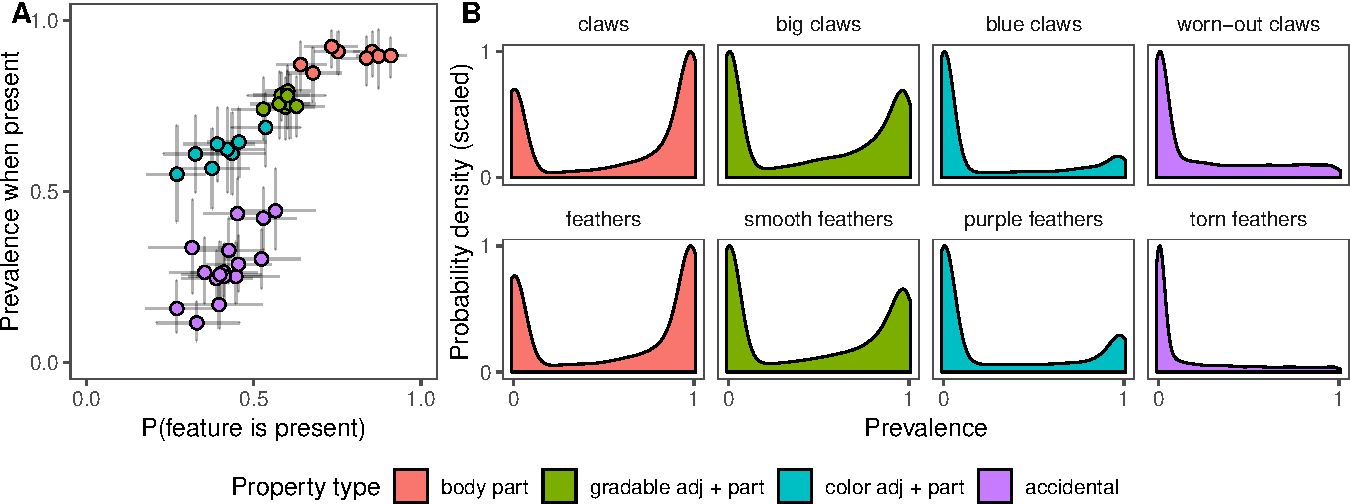
\includegraphics{genint_files/figure-latex/cimpian-prevPrior-1.pdf}
\caption{\label{fig:cimpian-prevPrior}Prevalence priors for items from
Cimpian et al. (2010). A: Latent parameters governing prevalence priors
are different for different kinds of properties. B: The diversity in
parameters gives rise to different underlying distributions over
prevalence, which the generic interpretation model uses to make
predictions.}
\end{figure}

\subsection{Experiment 1b: Generic
interpretation}\label{experiment-1b-generic-interpretation}

This experiment measures the prevalence implied by a generic statement
about a novel category, which we then compare to the predictions of the
generic interpretation model \(L(p \mid u)\) (Eq. \ref{eq:L0}).

\subsubsection{Method}\label{method-1}

\paragraph{Participants}\label{participants-1}

We recruited 40 participants over MTurk. The experimental design is very
similar to Cimpian et al. (2010), and we chose to have a sample size at
least twice as large as the original study (original n=15). This is a
quantitative experiment with only quantitative comparisons planned. All
participants were native English speakers. The experiment took about 5
minutes and participants were compensated \$0.60.

\paragraph{Procedure and materials}\label{procedure-and-materials-1}

In order to get participants motivated to reason about novel kinds, they
were told they were the resident zoologist of a team of scientists on a
recently discovered island with many unknown animals; their task was to
provide their expert opinion on questions about these animals.
Participants were supplied with a generic about a novel category (e.g.,
\enquote{Feps have yellow fur.}) and asked to judge prevalence:
\enquote{What percentage of feps do you think have yellow fur?}
Participants completed in randomized order 25 trials: 5 for each of the
biological properties and 10 for the accidental. The experiment in full
can be viewed at
\url{http://stanford.edu/~mtessler/generics/experiments/asymmetry/asymmetry-2.html}.

\subsubsection{Results}\label{results}

Figure~\ref{fig:cimpian-modelingResults} shows the prevalence implied by
the forty novel generic sentences in the experiment. We find a gradient
of interpretation, mostly clustered by the type of property. We first
explore a qualitative trend predicted by the interpretation model,
before proceeding to a quantitative model analysis. Prevalence implied
by a generic is predicted to vary according to the prevalence prior,
which we can summarize by its mean. We ran a Bayesian mixed-effects beta
regression model with fixed-effects of intercept and slope (scaled prior
mean) with random by-participant effects of intercept and slope. There
is a clear positive relationship between the prevalence prior mean and
the implied prevalence (\(\beta_{\text{prev prior mean}}=\) 0.704
{[}0.508, 0.919{]}).

\subsection{Model-based analysis and
results}\label{model-based-analysis-and-results}

\begin{figure}
\centering
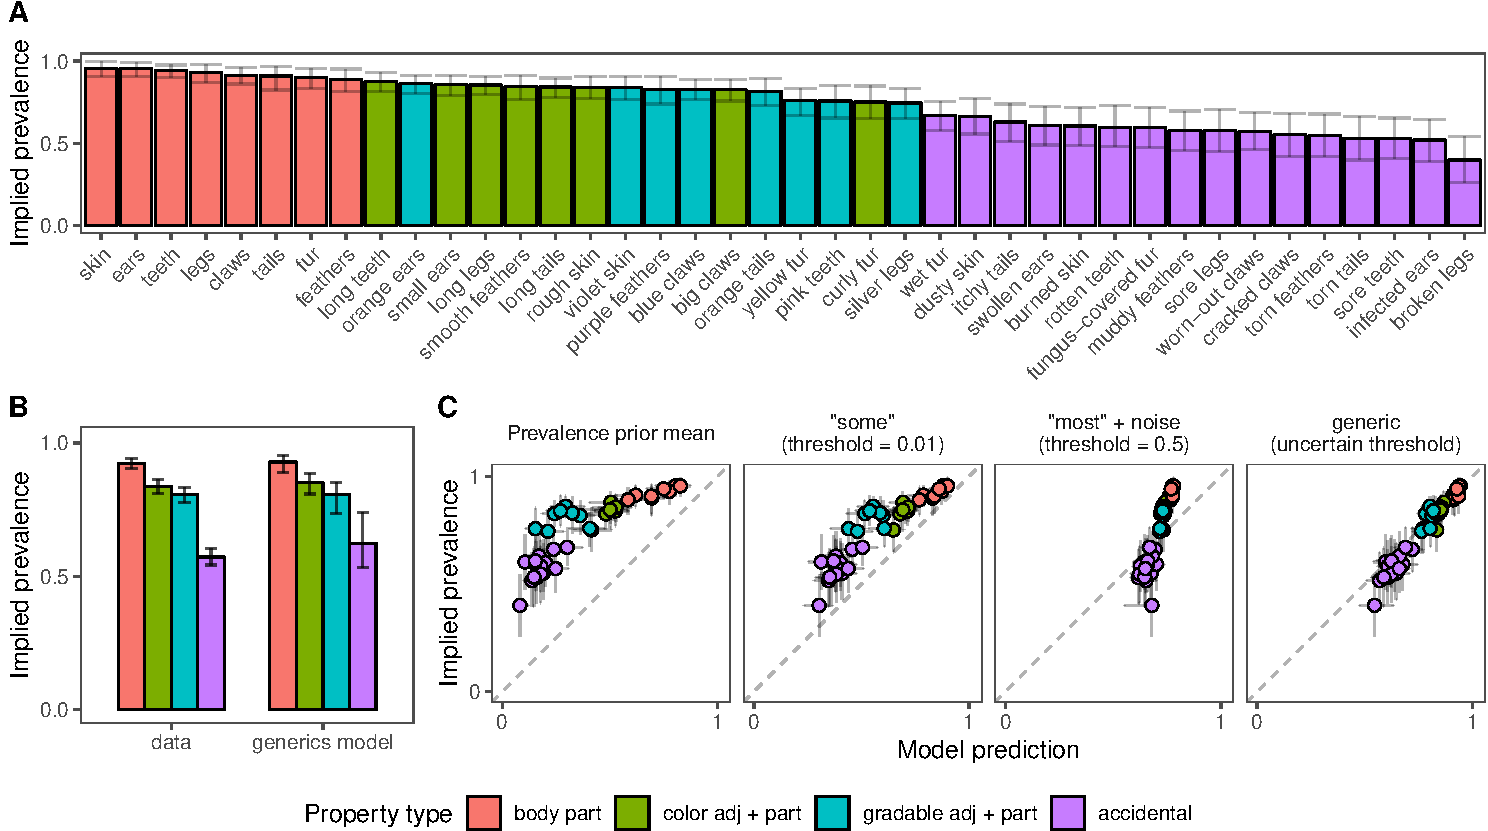
\includegraphics{genint_files/figure-latex/cimpian-modelingResults-1.pdf}
\caption{\label{fig:cimpian-modelingResults}Implied prevalence data and
model predictions for items from Cimpian et al. (2010). A: Mean implied
prevalence ratings for forty stimuli. B: Implied prevalence and generics
model prections collapsed across property type. C: Posterior predictive
model fits for quantitative models based on (i) the mean of the
prevalence prior, (ii) a threshold semantics fixed at 0.01
(\enquote{some}), (iii) a threshold semantics fixed at 0.5
(\enquote{most}), and (iv) an uncertain threshold semantics (generic).
Error bars denote bootstrapped 95\% confidence intervals for the
behavioral data and 95\% highest posterior density intervals for the
model predictions.}
\end{figure}

We now test the quantitative predictions of the model. We use the
prevalence priors inferred from Expt. 1a's structured elicitation task
as the prevalence prior \(P(r)\) in Eq. \ref{eq:L0} to predict the
generic interpretation data. We embedded our generic interpretation
model into the Bayesian data analysis model used to infer the priors; we
used the joint cognitive--data-analytic model to predict both the
prevalence prior data and the generic interpretation data
simultaneously. \ndg{that last sentence may confuse people?}
We ran the model using 3 chains of MCMC for 750,000 iterations, the first 250,000 of which were
discarded for burn-in. Figure~\ref{fig:cimpian-modelingResults}B shows
the generics model predictions and the human data for each of the four
types of properties (collapsing across items within a property-type). We
see that the model displays the same sensitivity to the kind of
property: Generics about body parts are interpreted the strongest,
accidental properties the weakest, with the other two types falling in
between.

We compare our generic interpretation to two lesioned versions of the
model, both of which lack the uncertain threshold. The first is a model
of the quantifier \enquote{some} which rules out the lowest possible
prevalence level. The second is analogous to \enquote{most}, with a
threshold at 50\% prevalence. However, a fixed threshold at 50\% is a
very restricted model; it places zero probability on any response less
than 50\%. Because there are many ratings in the data set that are less
than 50\%, we need to supplement the \enquote{most} model with an
extrinsic noise process in order for this model to actually generate
predictions for these data; with some probability, participants respond
at random. We infer this noise probability parameter from
the data.

Figure~\ref{fig:cimpian-modelingResults}C shows the model predictions in
the comparison to the behavioral data for each item independently for
the generics model, the two alternative fixed threshold models, and the
prevalence prior mean. The alternative models' defects are apparent
visually. The prevalence prior, though it is highly correlated with the
posterior (\(r^2(40)=\) 0.751), predicts too low values, resulting in a
high mean squared error (\(MSE=\) 0.151). The \enquote{some} model is
similar: It is highly correlated (\(r^2(40)=\) 0.855) but underpredicts
the data (\(MSE=\) 0.0349). The \enquote{most} + noise model achieves a
pretty good fit to the data (\(r^2(40) =\) 0.847; \(MSE=\) 0.0129), but
only does so because it predicts about a third of the data set is noise
(proportion noise = \(0.37 (0.33, 0.42)\)). Finally, the uncertain
threshold generic interpretation model explains practically all of the
variance in the data (\(r^2(40) =\) 0.953) and achieves an extremely low
mean squared error (\(MSE =\) 0.00229).

\subsection{Discussion}\label{discussion}

We replicated Cimpian et al. (2010)'s finding of a difference in the
implied prevalence between biological properties (e.g., \emph{yellow
fur}) and accidental properties (e.g., \emph{fungus-covered claws}). We
extended these findings with a broader stimulus set and discovered even
more gradability in interpretations of generic statements. We
empirically measured the prevalence priors and used our generic
interpretation model to predict prevalence implied by a generic
statement.

\ndg{it might be worth playing up the fact that structured elicitation of prevalence knowledge gives us a more detailed handle on what differs between these kinds of properties?}

The items that receive the lowest implied prevalence are those of
accidental or diseased states (e.g., \emph{fungus-covered claws},
\emph{broken legs}). As Cimpian et al. (2010) noted, \enquote{properties
of this type do not lend themselves very well to generic predication
(Cimpian \& Markman, 2008; Gelman, 1988), so generics about broken legs,
itchy skin, etc. are infrequent outside the laboratory.} (p.1472) It,
thus, remains a possibility that participants treat statements such as
\enquote{Lorches have broken legs} as an existential claim about the
here-and-now, analagous to how \enquote{Dogs are on my front lawn}
describes a particular state of affairs as opposed to something
generalizable about dogs. We thus aim to replicate these findings of low
prevalence interpretations in the next experiment, using properties that more naturally lend
themselves to generic interpretation.

\section{Experiment 2}\label{experiment-2}

This experiment is designed to measure the prevalence implied by a
generic about a diverse set of properties (Expt. 2b). In addition, we
elicit participants' beliefs about the likely prevalence levels expected
for these different properties (Expt. 2a). We again use our computational
model and alternative models, all using the elicited prevalence
priors, to make predictions about the prevalence implied by a generic.

\subsection{Experiment 2a: Prevalence prior
elicitation}\label{experiment-2a-prevalence-prior-elicitation}

\subsubsection{Methods}\label{methods}

\paragraph{Participants}\label{participants-2}

We recruited 144 participants from MTurk. This number was arrived at
with the intention of getting approximately 23 independent sets of
ratings for each unique item in the experiment. Participants were
restricted to those with U.S. IP addresses and with at least a 95\%
MTurk work approval rating (these same criteria apply to all experiments
reported). The experiment took on average 7.60 minutes and participants
were compensated \$0.80.

\paragraph{Materials}\label{materials}

We created a stimulus set composed of seventy-five properties. Items
were generated by the first author by considering six different classes
of properties: physical characteristics (e.g., \emph{have brown spots},
\emph{have four legs}), psychological characteristics (e.g.,
\emph{experience emotions}), dietary habits (e.g., \emph{eat human
food}), habitat (e.g., \emph{live in zoos}), disease (e.g., \emph{get
cancer}, \emph{carry malaria}), reproductive behavior (e.g., \emph{have
a menstrual cycle}), and other miscellaneous behaviors (e.g.,
\emph{pound their chests to display dominance}, \emph{perform in the
circus}); online sources about strange animal behaviors were consulted
in order to find the more obscure properties.

\ndg{materials in supplement / appendix}

\paragraph{Procedure and materials}\label{procedure-and-materials-2}

On the first trial, participants were asked to list three kinds of
animals for each of five different classes of animals: mammals, fish,
birds, insects/bugs, amphibeans/reptiles. The five classes of animals
were presented in a randomized order on the screen and there were three
text boxes for each in which participants could type an animal kind. On
subsequent trials, participants were shown a random subset of five
animal kinds and asked what percentage each of these categories they
believed had a property (e.g., \enquote{Out of all of the cheetas in the
world, what percentage do you think attack hikers?}). Pilot results
indicated similar responses were generated by a question about frequency
(e.g., \enquote{Out of 100 cheetahs, how many do you think attack
hikers?}). Participants responded using a slider bar with endpoints
labeled 0\% and 100\%, and the exact number corresponding to their
slider bar rating was displayed once participants clicked on the slider
bar. Each participant saw a random selection of twelve properties.

\ndg{say something about why elicitation paradigm is different for this expt than last one? partly to give a non-parametric look at priors?}

As an attention check, at the end of the prior elicitation trials,
participants were asked to select, from a list of ten, all of the
properties they could remember being tested on. The list included five
properties that they had been tested on and five distractors. The
experimental paradigm can be seen here:
\url{http://stanford.edu/~mtessler/generic-interpretation/experiments/generics/prior-3.html}.

\subsubsection{Results}\label{results-1}

We used the same exclusion criteria that were preregistered for the
subsequent generic interpretation study (Expt. 2b):
\url{https://osf.io/bwn4t/register/5771ca429ad5a1020de2872e}.
Participants who did not have at least 4 out of 5 hits and at least 4
out of 5 correct rejections during the memory trial were excluded
(\(n = 10\)). In addition, we excluded participants who self-reported a
native language other than English (\(n = 9\)). This left a total of
\(n = 126\) participants, with items receiving on average 20 (range =
{[}11, 29{]}) unique participants responses (each participant provides
five ratings).

A response in this task can be thought of as a sample from a property's
prevalence prior distribution. Thus, the distribution of responses for
an item are an estimate of the prevalence prior distribution.
Figure~\ref{fig:genInt-prevPrior}A shows eight example items'
distributions of responses. The property \emph{have four legs} is most
likely either completely present (prevalence = 100\%) or completely
absent (prevalence = 0\%) from categories. \emph{Eat insects} looks
similar, though there is considerable probability mass spread among the
non-binary alternatives (\(0\% <\) prevalence \(< 100\%\)). \emph{Get in
fights with other animals} has substantial less probability mass at
100\% prevalence: It is unlikely that this property is widespread in a
category. \emph{Live in urban areas} shows a monotonically decreasing
probability function; the higher the prevalence, the less likely it is.
\emph{Live in zoos} is expected to be even less prevalent, and the
property \emph{has seizures} is expected to not be widespread at all.
The property \emph{get erections} is only expected to be present in 50\%
of the population (presumably, the males) when it is present at all.

Most of the elicited prevalence prior distributions are at least
bi-modal. To visualize all properties simultaneously, we represent each
distribution by its relative probability mass at
0\%---\(P(\text{feature is present})\), or \(P(r > 0)\)---and the
expected value (mean) of the distribution conditional on the prevalence
being greater than 0\%---\(\mathbb{E}[P(r \mid r>0)]\), which we refer
to as \emph{prevalence when present}
(Figure~\ref{fig:genInt-prevPrior}B). Our stimulus set covers a wide
range of possible values of both of these parameters; the set of
parameters that summarize these priors is also largely non-overlapping
with those of Expt. 1 (compare with
Figure~\ref{fig:cimpian-prevPrior}A). This suggests we have sampled
items with priors that exhibit a lot of quantitative variability. Given
these priors, our model makes quantitative predictions about the
prevalence implied by a novel generic sentence (e.g., \enquote{Lorches
live in zoos}).

\begin{figure}
\centering
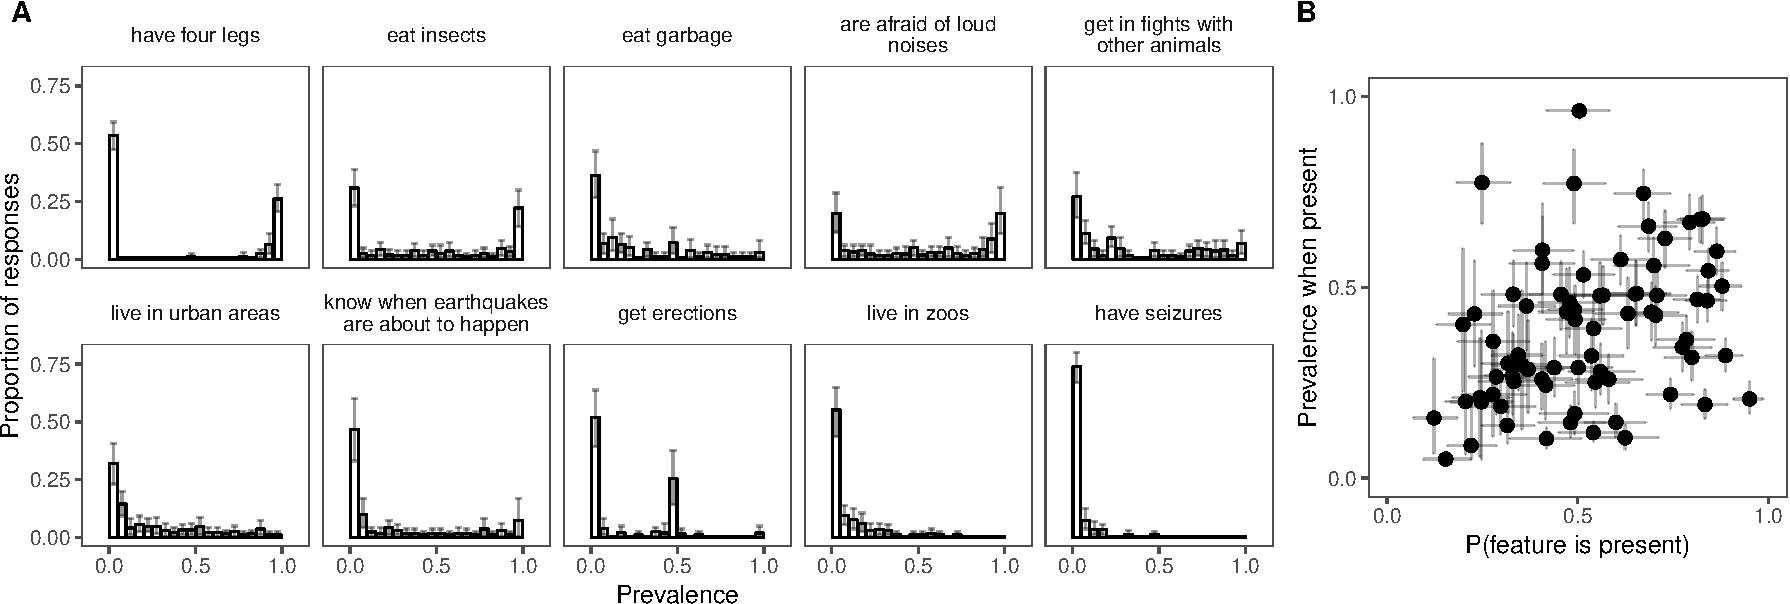
\includegraphics{genint_files/figure-latex/genInt-prevPrior-1.pdf}
\caption{\label{fig:genInt-prevPrior}Prevalence priors for a broad set of
animal properties. A: Ten example prevalence priors elicited in Expt.
2a. Different prevalence priors give rise to different model predicted
implied prevalence. B: Prevalence priors summarized by their relative
probability mass at zero-prevalence P(feature is present), and their
expected value among non-zero prevalence levels: Prevalence when
present. Error bars denote bootstrapped 95\% confidence intervals.}
\end{figure}

\subsection{Experiment 2b: Generic
interpretation}\label{experiment-2b-generic-interpretation}

\subsubsection{Methods}\label{methods-1}

\paragraph{Participants}\label{participants-3}

We recruited 200 participants from MTurk. This number was arrived at
with the intention of getting approximately 50 ratings for each unique
item in the experiment. The experiment took on average 5.50 minutes and
participants were compensated \$0.80.

\paragraph{Procedure and materials}\label{procedure-and-materials-3}

The materials were the same as in Expt. 2a. Participants were told that
scientists had recently discovered lots of new animals that we did not
know existed. On each trial, they would be told facts about the new
animals and be asked to translate it into the percentage of that animal
it applies to. On each trial, participants read \enquote{You are told:
\emph{generic sentence}}, where the generic sentence was a bare plural
statement about a familiar property \(F\) applying to a novel animal
category \(K\) (e.g., \enquote{Javs attack hikers}). They were then
asked \enquote{Out of all of the \emph{K}s on the planet, what
percentage do you think \emph{F}?} (e.g., \enquote{Out of all of the
javs on the planet, what percentage do you think attack hikers?}). Novel
animal category names were mostly taken from Cimpian et al. (2010) and
similar studies on generic language. Participants responded using a
slider bar with endpoints labeled 0\% and 100\%, and the exact number
corresponding to their slider bar rating was displayed once participants
clicked on the slider bar. Each participant completed thirty-five
trials, corresponding to a random subset of the full stimulus set.

After the generic interpretation trials, participants completed the same
memory check trial as was done in the prior elicitation. They were shown
ten properties and asked to click on those they had seen in the
experiment. Following the memory check trials and depending on their
ratings in the task, participants completed up to five explanation
trials. On an explanation trial, participants saw a rating they had
given for a property they had rated as applying to less than 50\% and
asked if they could explain why they gave the response that they gave.
Participants also had the option of changing their response after
providing an explanation. (These data were used in an exploratory
analysis.) If participants gave no ratings less than 50\%, they did not
complete any explanation trials.

The experiment paradigm can be viewed at
\url{http://stanford.edu/~mtessler/generic-interpretation/experiments/generics/interpretations-6.html}

\subsubsection{Results}\label{results-2}

We used preregistered exclusion criteria, which were also used for Expt.
2a. Participants who did not have at least 4 out of 5 hits and at least
4 out of 5 correct rejections during the memory trial were excluded
(\(n = 62\)). In addition, we excluded participants who self-reported a
native language other than English (\(n = 8\)). This left a total of
\(n = 132\) participants, with items receiving on average 62 responses
(range = {[}50, 77{]}).

To assess the reliability of these data, we ran a replication
(\(n=140\)) using a slightly different dependent measure.\footnote{By
  experimenter error, only seventy-four of the seventy-five items were
  collected in the replication data set.} Instead of being asked a
question about percentages (e.g., \enquote{Out of all of the Ks in the
world, what percentage F?}), participants were asked a question in terms
of frequency: \enquote{Out of 100 Ks, how many do you think F?}. The
empirical by-item means between these data and the original data are
highly correlated (\(r(74) = 0.96\), \(r_{spearman}(74)= 0.96\)),
indicating very high data reliability.

\paragraph{Descriptive results}\label{descriptive-results}

Interpreting a novel generic sentence \enquote{Ks have F} often has the
possibility of being understood as a universal claim (\emph{all or
almost all Ks Fs)}. Across our seventy-five items, however, we observe a
clear gradient in the implied prevalence ratings
(Figure~\ref{fig:genint-modelingResults}A). On one end of the continuum,
we have the generic \enquote{Wugs have four legs}, which is interpreted
as a universal---applying to exactly 100\% of wugs---by 36 out of 70
participants and which received a mean implied prevalence rating of
\(0.96 [0.93, 0.98]\).\footnote{Note the novel category term is
  randomized for each participant and property. We use particular novel
  category terms in the text for ease of exposition.} On the other end
is \enquote{Glippets perform in the circus}, which is interpreted as
applying to less than 25\% of glippets by 35 out of 61 participants and
which receives a mean rating below 50\% (\(0.31 [0.23, 0.39]\)).
Additionally remarkable is the distribution of responses for individual
items: Though \enquote{Feps live in zoos} probably means around 25\% of
feps live in zoos, it is still quite possible that almost 100\% live in
zoos (e.g., in the real world, 100\% of Micronesian Kingfishers live in
zoos).

Several properties about the reproductive behavior of animals have
interpretation distributions that are bimodal. For example,
\enquote{Morseths have a menstrual cycle} is interpreted primarily as
applying to 50\% of morseths (38 out of 64 give a response between 45\%
and 55\%); however, some participants (10 of 64) rate this as applying
to 100\% of morseths.\footnote{The scientifically correct term for this
  is actually an \enquote{estrous cycle}. We are grateful to one of our
  MTurk participants for pointing this out to us.} 
  
  \ndg{move this to a discussion section:}This behavior could
result from a participant interpreting the question as pragmatically
restricting the domain to only the members of that category that
\emph{could} have the property (e.g., 100\% of female morseths have a
menstrual cycle). We notice this bimodal interpretation in our
prevalence elicitation task (Expt. 2a) as well: The distribution over
several of the reproductive properties is tri-modal, with peaks at 0\%
(the animals that don't have a menstrual cycle), 50\% (\enquote{only
females}) and 100\% (perhaps, \enquote{all females}). The fact that this
multi-modality appears in the prior elicitation task as well means that
the generic interpretation model will be well-positioned to predict a
bi-modal distribution for the implied prevalence data.

\paragraph{Model-based analysis and
results}\label{model-based-analysis-and-results-1}

Our primary analysis concerns how well the uncertain threshold generic
interpretation model can accomodate the implied prevalence data in
comparison to alternative models. To fit these models, we construct a
Bayesian data analysis (BDA) model to jointly predict the prevalence
prior data (Expt. 2a) and the generic interpretation data (Expt. 2b).
Such a joint-inference mode allows us to retain the uncertainty in the
measurement of the prevalence prior data when using it in our model to
predict the implied prevalence results. \ndg{that last sentence is very clarifying. put it (also) in expt 1 analysis section?}

The joint cognitive-statistical model attempts to predict both data
sources (prevalence prior and generic interpretation) simultaneously;
the former is modeled as a mixture of three Beta distributions and the
latter is modeled by our generic interpretation model (Eq. \ref{eq:L0}).
Beta is an appropriate choice for the prevalence prior data because it
is a distribution over numbers on the unit interval (the same as our
slider ratings), and we allow each individual property's prevalence
prior to be composed of up to three constituent Betas to allow the
statistical model the flexibility to accomodate the complex prevalence
prior distributions. Each prevalence prior, thus, has eight parameters
governing its shape: a mean \(\gamma\) and variance parameter \(\xi\)
for each of the three Beta components and two parameters \(\phi_1\),
\(\phi_2\) that describe the relative weighting among the three
components. We put uninformative priors over these parameters
\(\gamma \sim \text{Uniform}(0, 1)\),
\(\xi \sim \text{Uniform}(0, 100)\),
\(\phi \sim \text{Dirichlet}(1,1,1)\). The inferred prevalence prior
distributions are then used as \(P(r)\) in Eq. \ref{eq:L0} in order to
generate predictions for the generic interpretation data.\footnote{In
  reality, this procedure is done simultaneously, not sequentially.} The
generic interpretation model is fully specified by Eq. \ref{eq:L0} and
has no free parameters. The model is implememented in the probabilistic
programming language WebPPL (Goodman \& Stuhlmüller, 2014).

\ndg{it seems like there is a lot of duplication between this data analysis section and that of expt 1, and also that it's kind of long given its location in the narrative. how about a section after model, before expts, outlining our data analysis approach (jointly modeling prior data and interpretation data using beta mixtures and such)?}

To learn about the credible values of the parameters governing the
prevalence priors as well as generate model predictions for the generic
interpretation data, we performed Bayesian inference on the model by
running three chains of an incrementalized version of MCMC (Ritchie,
Stuhlmüller, \& Goodman, 2016) for 750,000 iterations, removing the
first 250,000 iterations for burn-in. A qualitative examination showed
that the prevalence prior distributions were well-modeled as a mixture
of three Beta distributions. Often one Beta distribution is devoted to
accounting for the very small numbers (0\% or near 0\% prevalence
ratings), while the two other components model the other parts of the
distribution, the details of which depend upon the property.

As a first attempt to understand the implied prevalence data in a
quantitative way, we compare the means of the inferred prevalence priors
to the empirical means of the implied prevalence data
(Figure~\ref{fig:genint-modelingResults}B top facet). The means of the
prevalence prior distributions do a rather poor job at predicting the
implied prevalence ratings, consistently underpredicting the ratings
(\(r^2(75) = 0.59\), \(MSE = 0.24\)). The fact that the prevalence prior
data does not fit the generic interpretation data is good evidence that
participants are actually \emph{updating} their beliefs about the
property in the generic interpretation task, as opposed to simply
responding according to their prior beliefs.

We ran alternative interpretation models using the same data analytic
approach (i.e., joint cognitive-statistical models) but which had access
to only a single fixed-threshold rather the uncertain threshold of the
generic interpretation model.
\ndg{similarly, a short section on alternative models at the end of the model section would save having to re-explain the alternatives each time, and give a better flow.}
 These alternative models correspond to
models of the quantifier \enquote{some} and \enquote{most} and provide
strict tests of our generic interpretation model because they too have
access to the full prior distribution over prevalence as well as the
flexibility endowed by the Bayesian data analysis method.
Figure~\ref{fig:genint-modelingResults}B shows each of the alternative
model's predictions (technically, the BDA models' posterior predictive
distributions) for the mean implied prevalence of each of the
seventy-novel generic sentences, in comparison to the empirical means.
We see that the model based on quantifier \enquote{some} (i.e., a fixed
threshold at the lowest possible value) consistently
\emph{underpredicts} the implied prevalence, consistent with the
intuition that assigning the semantics of \enquote{some} for generics is
too weak. Though the model explains a lot of the variance
\(r^2(75) = 0.91\), it does so with a relatively high mean squared error
\(MSE = 0.038\).

It is impossible for the model based on the quantifier \enquote{most} to
accomodate these data: \emph{Most} has a strict threshold at 0.5 and
thus assigns probability 0 to all responses less than 0.5. \ndg{you said this already in expt 1} In order to
alleviate this issue, we endow the BDA model for \enquote{most} with a
external noise parameter, which allows the model to randomly guess on
some proportion of trial (the exact proportion is a parameter to be
inferred from the data). The \enquote{most} model assigns 0.57 {[}0.55,
0.59{]} proportion of the data to be noise, because of the high
prevalence of minority (i.e., less than 50\%) interpretations. A model
based on the semantics for \enquote{most} is not well-suited for these
data \(r^2(75) = 0.49\), \(MSE = 0.021\).

Finally, we examine the uncertain threshold model's predictions for the
mean implied prevalence ratings. Unlike each of the alternative models,
the uncertain threshold is able to perfectly accomodate the highly
variable generic interpretation data \(r^2(75) = 0.97\),
\(MSE = 0.0025\). The generic interpretation model is able to flexibly
adjust the threshold depending on the prevalence prior, resulting in
context-sensitive generic interpretation that finely tracks human
judgments.

\begin{figure}
\centering
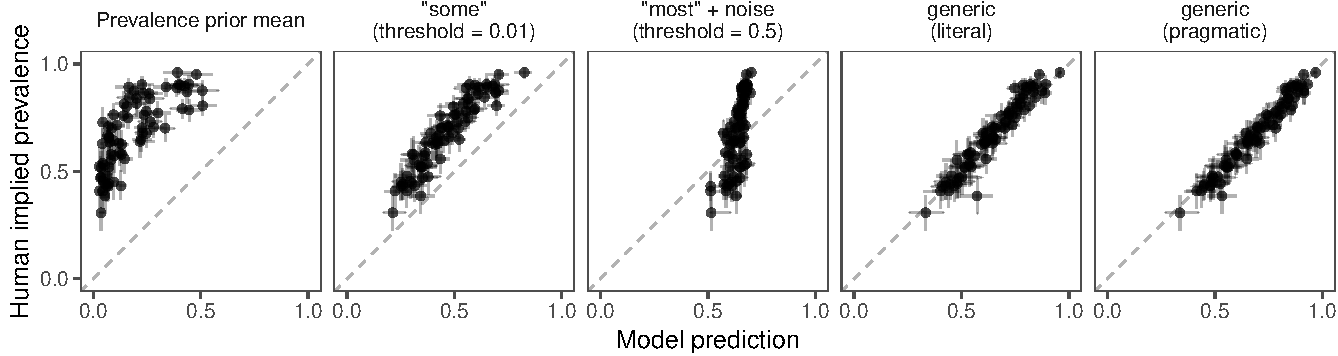
\includegraphics{genint_files/figure-latex/genint-modelingResults-1.pdf}
\caption{\label{fig:genint-modelingResults}Implied prevalence data and model
predictions for a broad set of seventy-four items. A: Mean implied
prevalence ratings (points are individual empirical judgments). B:
Posterior predictive model fits for quantitative models based on (i) the
mean of the prevalence prior, (ii) a threshold semantics fixed at 0.01
(\enquote{some}), (iii) a threshold semantics fixed at 0.5
(\enquote{most}), and (iv) an uncertain threshold semantics (generic).
The model for \enquote{most} is outfitted with a noise parameter to
accomodate data points that are logically impossible given the fixed
semantics. Error bars denote bootstrapped 95\% confidence intervals for
the behavioral data and 95\% highest posterior density intervals for the
model predictions.}
\end{figure}

\section{Experiment 3: Prior
Manipulation}\label{experiment-3-prior-manipulation}

In the previous experiments, we see how participants' prior beliefs
about the prevalence of the property, either measured by asking about
alternative categories (Expt. 2) or abstract questions about the
distribution of the property (Expt. 1), related to the prevalence
implied by a novel generic via a model that reasons about an uncertain
threshold on prevalence (Eq. \ref{eq:L0}). In both of the previous
experiments, we measured both generic interpretation and the prevalence
prior and related the two via our model. Though our model is able to
finely track interpretations in a way that alternative models cannot,
the evidence so far for the influence of the prevalence prior on
interpretation is merely correlational. We have shown that the two are
related but not that intervening on the prevalence prior can change
interpretations.

In this final experiment, we test the causal role of the prevalence
prior in generic interpretation. We do this by manipulating the
prevalence prior and measuring the resulting influence on interpretation
(\emph{generic interpretation} condition). To serve as a manipulation
check, we first elicit predictions about prevalences following our prior
manipulation procedure; these predictions also serve as the measurements
of the (manipulated) prevalence priors used in our model.

\subsection{Experiment 3a: Prior elicitation (manipulation
check)}\label{experiment-3a-prior-elicitation-manipulation-check}

\subsubsection{Methods}\label{methods-2}

\paragraph{Participants}\label{participants-4}

We recruited 200 participants from MTurk. This number was arrived at
with the intention of getting approximately 30 ratings for each unique
item in the experiment. The experiment took on average 3 minutes and
participants were compensated \$0.30.

\paragraph{Materials}\label{materials-1}

The goal of this experiment was to manipulate the prevalence prior. To
focus on the influence of our prior manipulation cover story (described
below), we chose to use a single property (\emph{know when earthquakes
are about to happen}) whose prevalence prior elicited in Expt. 2a
suggested participants had a lot of uncertainty as to what prevalence
levels to expect for this property, and thus could be particularly
amenable to manipulation.\footnote{Pilot testing using a completely
  novel property (e.g., \emph{daxing}) appeared to make the task too
  artificial. Participants seemed to treat the task as a number game.}

Participants were familiarized with one of ten prevalence prior
distributions, shown in Figure~\ref{fig:priorManipulationExpt}E). Nine
of the ten distributions are bimodal with modes either at 0\%, 25\%,
50\%, 75\%, or 100\%; the tenth distribution is uniform over all
prevalence levels between 0\% and 100\%. The mixture between
the two modes was always 50\% (half of samples were from one mode and
half from the other, as shown in
Figure~\ref{fig:priorManipulationExpt}B).

\paragraph{Procedure}\label{procedure}

\begin{figure}
\centering
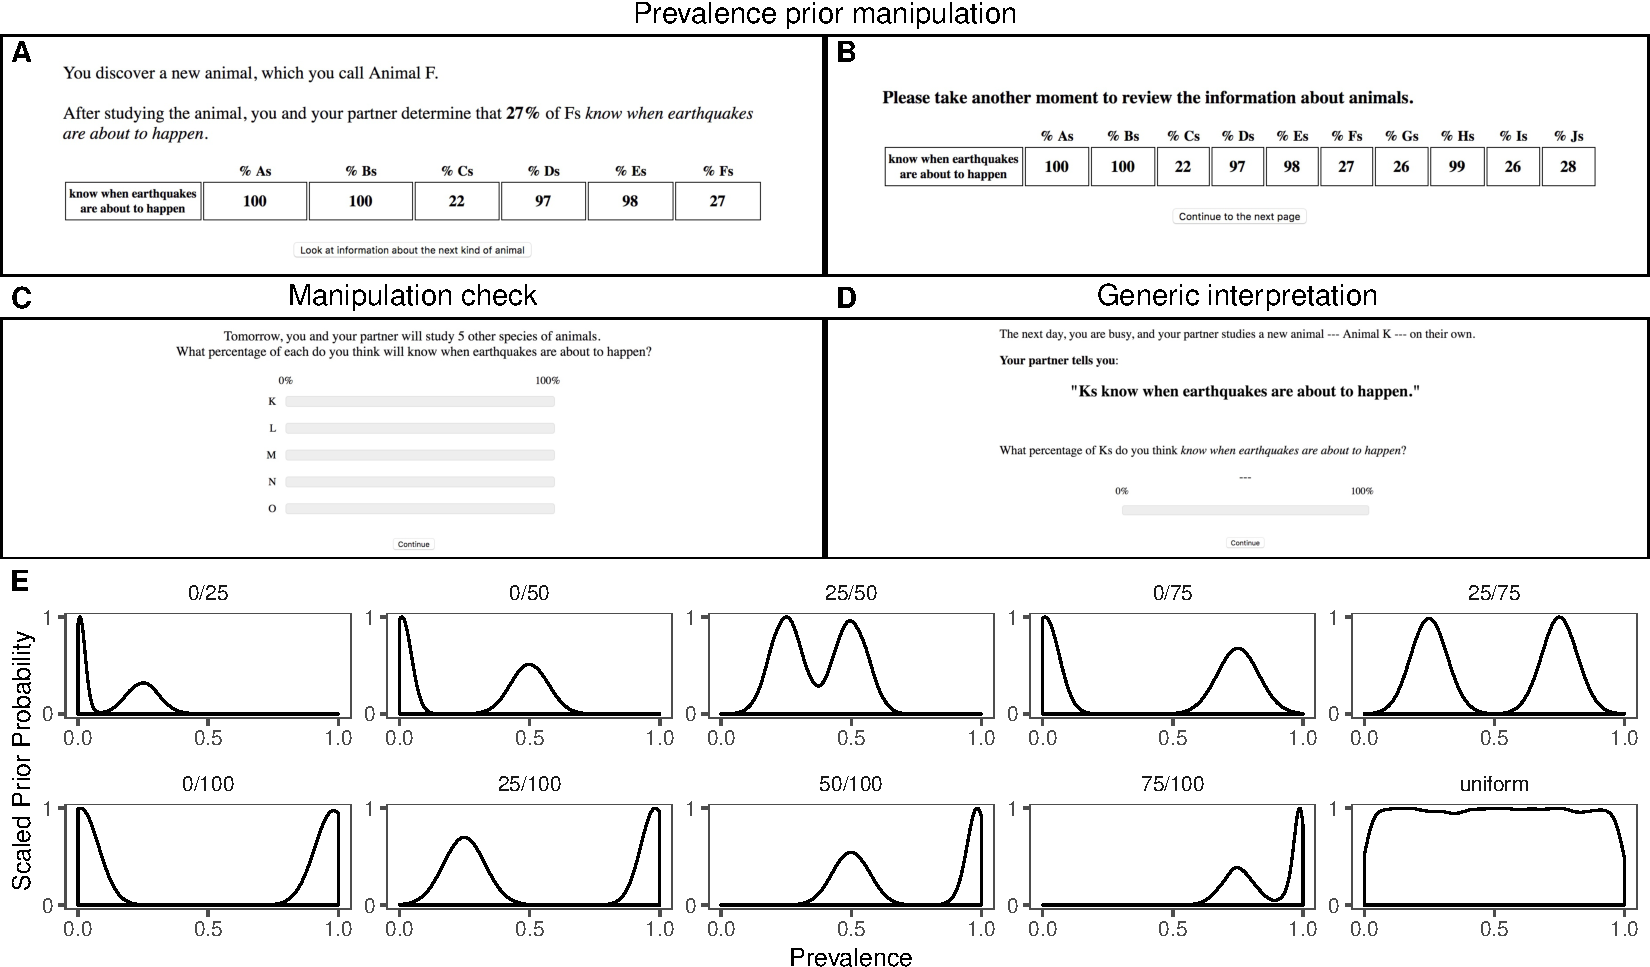
\includegraphics{genint_files/figure-latex/priorManipulationExpt-1.pdf}
\caption{\label{fig:priorManipulationExpt}Overview of Experiment 3. A:
Prevalences of feature in animals are shown one at a time, described in
text and displayed in a table. B: Participants are asked to review
previous results once all displayed. C: Prior elicitation task:
Participants predict the results of the next five animals. D: Generic
interpretation task: Participants rate prevalence after reading generic
sentence. E: Experimentally manipulated prevalence prior distributions.
The distribution shown in B is the \emph{weak or deterministic}
distribution.}
\end{figure}

In order to avoid participants learning the structure of the task,
participants completed only a single trial: Each participant saw only
one prevalence distribution. Participants were given a cover story in
which they were asked to imagine they were an astronaut-scientist
exploring a distant planet with lots of new animals on it. They were
studying these animals with another scientist to understand the animals'
ability to \enquote{know when earthquakes are about to happen}.
Participants were then shown data that they and their fellow scientist
had collected about the prevalence of the property among different novel
animals. In order to minimize distraction, novel animals were simply
labeled by a letter (e.g., \enquote{Animal C} or just \enquote{Cs}).
Information about the animal appeared in an \emph{evidence statement}
(e.g., \enquote{After studying the animal, you and your partner
determine that 98\% of Cs \emph{know when earthquakes are about to
happen}.}) and were displayed in a table showing the corresponding
numerical data (Figure~\ref{fig:priorManipulationExpt}A). Participants
proceed in a self-paced way by clicking a button to reveal information
about the next animals. After participants viewed the data for ten
categories, they are told to review the information about the animals
before continuing (Figure~\ref{fig:priorManipulationExpt}B). Then, the
data table is removed and participants are provided the following
prompt:

\begin{quote}
Tomorrow, you and your partner will study 5 other new species of
animals. What percentage of each do you think will know when earthquakes
are about to happen?
\end{quote}

Participants were given five slider bars ranging from 0\% - 100\%, and
asked to predict the prevalence for the next five categories (Animals K
- P; Figure~\ref{fig:priorManipulationExpt}C). After rating the slider
bars, participants were asked if they could explain why they gave the
responses that they did. Then, they completed an attention check survey
where they were asked what property was being investigated (choosing a
response from a list of 10 options) and to input one of the prevalence
levels they saw on the familiarization screen.

\subsubsection{Results}\label{results-3}

Participants who failed to either select the correct property or list a
correct number from the familiarization period were excluded.

Similar to the data from Expt. 2a, a response in this task can be
thought of as a sample from a prevalence prior distribution and the
distribution of responses as estimates for the whole distribution. We
visualize the distributions by discretizing the responses so that each
response goes into one of twenty equally spaced bins (effectively
turning the 101-pt scale into a 20-pt scale).
Figure~\ref{fig:priorManipulationResults}A (top row) shows the
empirically elicited predicted prevalence distributions. These
distributions clearly reflect the familiarization distributions supplied
to participants in the experiment, with some idiosyncractic features.
The distribution that is most different from the familiarization
distribution is the uniform distribution; the empirical predicted
distribution is more unimodal with a peak at 50\%. Many distributions
exhibit a regression to the mean in some participants' predictions: In
the \emph{rare or deterministic} distribution (which featured prevalence
levels either around 0\% or 100\%), some participants guess that the
next animal will have 50\% prevalence; a similar phenomenon can be
observed in the \emph{weak or strong} distribution (25\% or 75\%) and to
a lesser extent in the other bimodal distributions.

Because our generic interpretation model has no free parameters, we use
these empirically measured prevalence distributions to generate \emph{a
priori} model predictions using the generic interpretation data. To
account for our uncertainty in the measurement of the prevalence priors,
we bootstrap the priors by resampling subjects (with replacement),
calculating the empirical prevalence distributions (by binning, as
above), and generating model predictions. We repeated this procedure
10,000 times to generate distributions of predictions. The boostrapped
mean and 95\% quantiles for each prevalence bin in each distribution are
shown in Figure~\ref{fig:priorManipulationResults}A (middle row). We see
that context-sensitive interpretations are predicted, with
idiosyncracies that reflect empirically measured distributions. We then
tested these predictions against interpretations in the same empirical
paradigm.

\begin{figure}
\centering
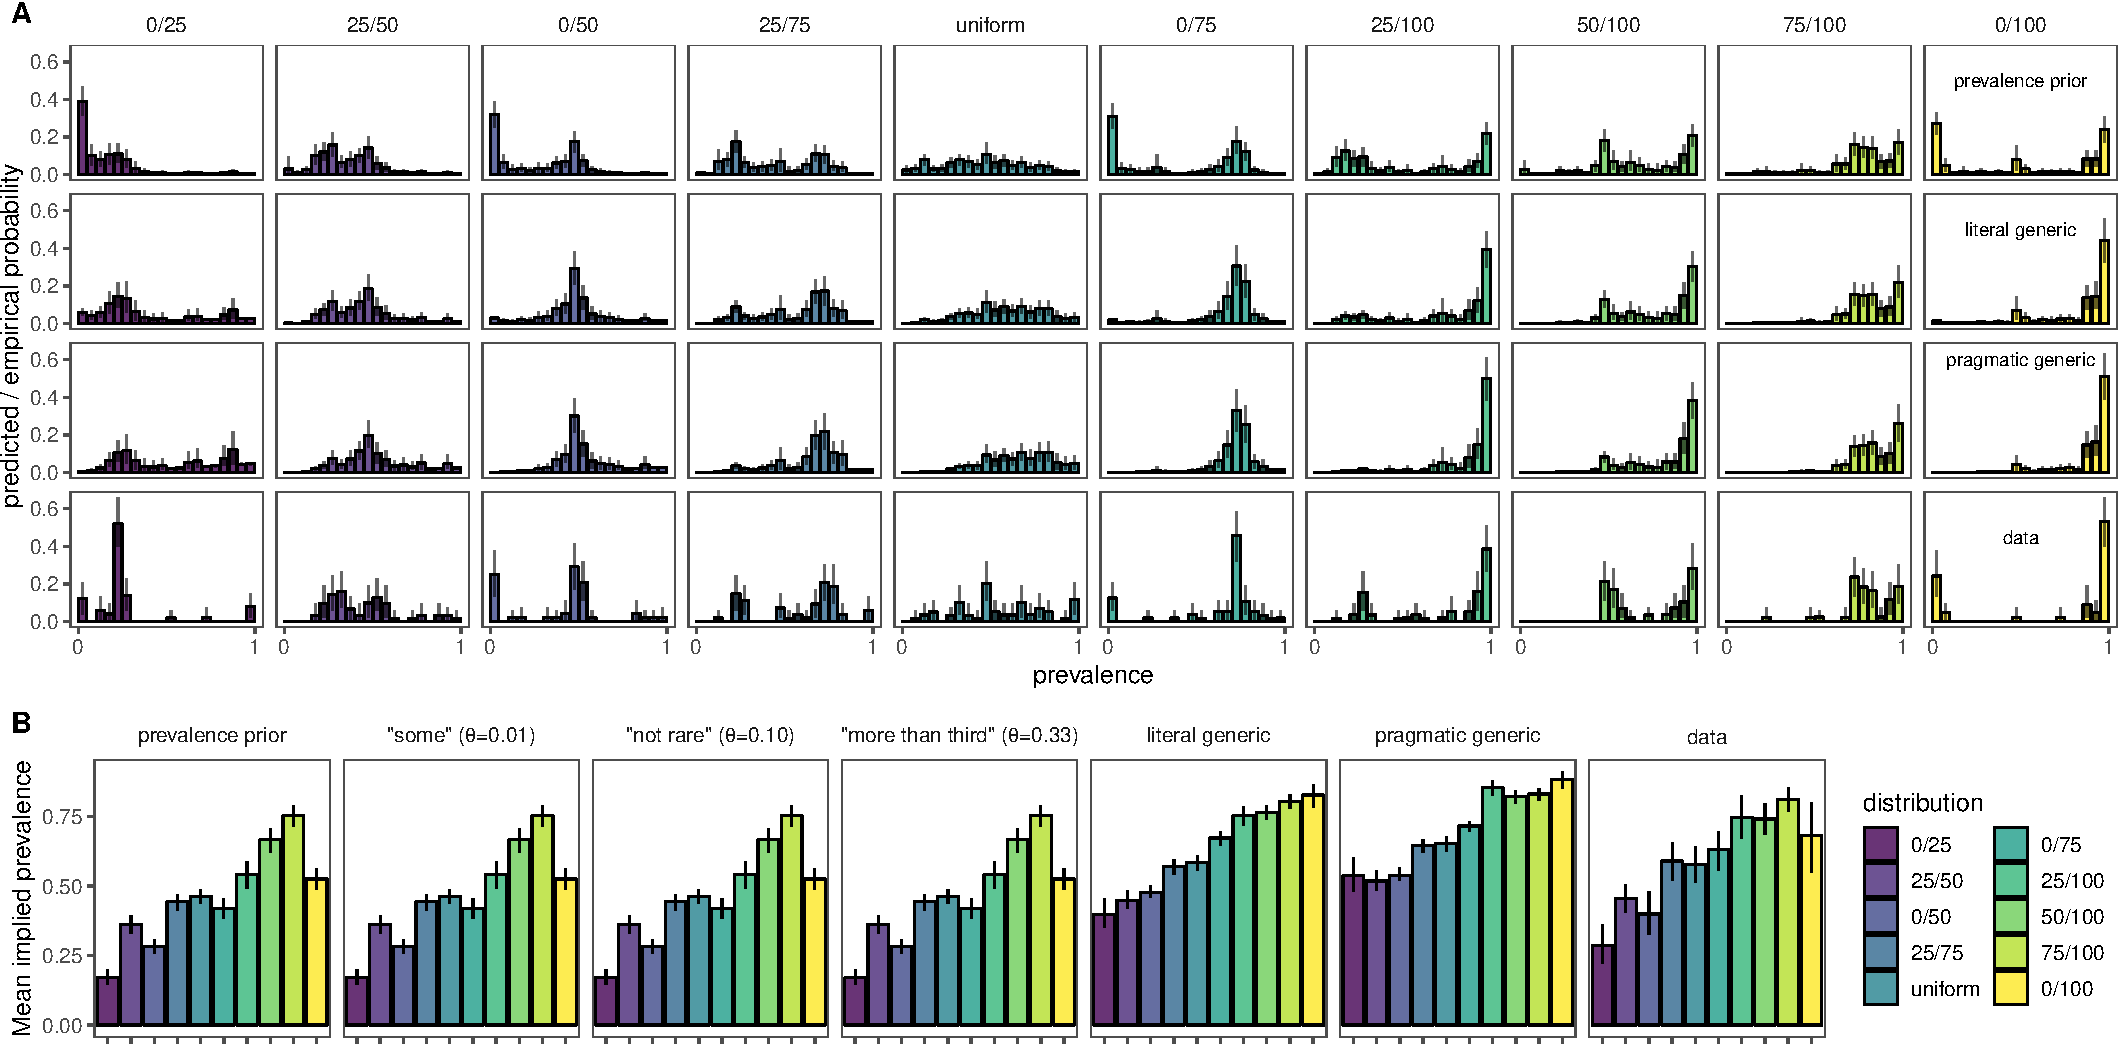
\includegraphics{genint_files/figure-latex/priorManipulationResults-1.pdf}
\caption{\label{fig:priorManipulationResults}Experiment 3 results. A:
Empirical distribution of responses for the prior elicitation task
(Expt. 3a), generics model predictions based on those empirical
distributions, and empirical distributions of responses for the generic
interpretation task (Expt. 3b). B: Model predicted means for several
alternative models and empirical means. C: Same as B shown in
scatterplot. \ndg{why show both ways? also, fix label cut off in C.}}
\end{figure}

\subsection{Experiment 3b: Generic
interpretation}\label{experiment-3b-generic-interpretation}

\subsubsection{Methods}\label{methods-3}

The sample size, exclusion criteria, and planned statistical contrasts
were all preregistered:
\url{https://osf.io/n342q/register/5771ca429ad5a1020de2872e}.

\paragraph{Participants}\label{participants-5}

We recruited 600 participants from MTurk. This number was arrived at
with the intention of getting approximately 50 ratings for each unique
item in the experiment. The experiment took on average 2.70 minutes and
participants were compensated \$0.30.

\paragraph{Materials and procedure}\label{materials-and-procedure}

The materials and procedure were identical to those of Expt. 3a with the
following exception. After the familiarization period, the data table is
removed and participants are provided the following prompt:

\begin{quote}
The next day, you are busy and your partner studies a new animal on
their own: Animal K. Your partner tells you: \enquote{Ks know when
earthquakes are about to happen.}
\end{quote}

In order to encourage participants to pay attention to the language,
this text is on the screen for five seconds before participants are
asked: \enquote{What percentage of Ks do you think know when earthquakes
are about to happen?} and provided with a slider bar ranging from
0\%-100\% (Figure~\ref{fig:priorManipulationExpt}D). As in Expt. 3a,
participants then completed an attention check survey where they were
asked what property was being investigated and to input one of the
prevalence levels they saw on the familiarization screen. The experiment
can be viewed at
\url{http://stanford.edu/~mtessler/generic-interpretation/experiments/generics/prior-manipulation-2.html}.

\subsubsection{Results}\label{results-4}

We used preregistered exclusion criteria, which were also used for Expt.
3a. Participants who failed to either select the correct property or
list a correct number from the familiarization period were excluded
(\(n = 39\)). In addition, we excluded participants who self-reported a
native language other than English (\(n = 33\)). This left a total of
\(n = 532\) participants, with items receiving on average 53 responses
(range = {[}43, 62{]}).

Our main qualitative hypothesis is that there would be a difference
across conditions in interpretations of the same generic sentence
(\enquote{Ks know when earthquakes are about to happen}). The
differences in interpretations are evident in the empirical
distributions of responses (Figure \ref{fig:priorManipulationResults}A,
bottom row). More specifically, we predict that the prevalence implied
by the generic sentence will, to a first approximation, track the mean
of the prevalence prior distribution. To test this, we ran a linear
model predicting responses with a fixed effect of the prior mean (as
estimated by the data from Expt. 3a). There was a significant main
effect of prior mean, with a coefficient close to 1 (\(\beta_1 = 0.94\),
\(SE=0.07\), \(t = 12.76\)), indicating a strong linear relationship
between the mean of the learned prevalence prior and the resulting
interpretations. Furthermore, there was a significant main effect of
intercept, indicating that participants' responses were significantly
greater than the mean of the corresponding prevalence priors
(\(\beta_0 = 0.16\), \(SE=0.04\), \(t = 4.44\)). These results show that
participants interpret the novel generic sentence in a manner sensitive
to the background distribution and that the generic utterance updates
participants' beliefs to indicate a prevalence significantly higher than
the prior. There is a lot more to be learned from these data, however;
this simple linear model explains less than a quarter of the variance in
the data \(r^2 = 0.24\).

From the generics model, we are able to make a number of \emph{a priori}
predictions about quantitative differences in mean implied prevalence
ratings across the ten conditions. These predictions were derived by
examining pairs of conditions with small quantitative differences but
for which the bootstrapped 95\% confidence interval around the generics
model predictions did not overlap
(Figure~\ref{fig:priorManipulationResults}B, \enquote{generics model}
panel). With those criteria in mind, we preregistered the following
contrast predictions among mean implied prevalences (\{\}s indicate no predicted difference): 0/25
\(<\) \{25/50, 0/50\} \(<\) \{25/75, \emph{uniform}\} \(<\) 25/75 \(<\)
\{25/100, 50/100\} \(<\) \{75/100, 0/100\}. To evaluate these
predictions, we built a Bayesian regression model with the relevant
contrasts using a \enquote{zero and one inflated beta} linking function
to appropriately model the responses of exactly 0\% and 100\%, which are
undefined under the beta distribution. The maximum a-posteriori
estimates and 95\% credible intervals of the coefficients of the
regression model, as well as the model predicted qualitative
differences, are shown in Table 1. Each of the five predicted positive
differences were estimated to be greater than zero, and each of the four
predicted null differences were not different from zero.

\begin{table}[h]
\centering
\begingroup\fontsize{9pt}{10pt}\selectfont
\begin{tabular}{llrl}
  \hline
coefficient & prediction & Estimate & credible\_interval \\ 
  \hline
Intercept &  & 0.32 & [ 0.221, 0.418] \\ 
  0/25 vs. \{25/50, 0/50\} & $>$ & 0.15 & [ 0.036, 0.278] \\ 
  25/50 vs. 0/50 & = & -0.07 & [-0.270, 0.134] \\ 
  \{0/25, 25/50, 0/50\} vs. \{25/75, uniform\} & $>$ & 0.34 & [ 0.265, 0.409] \\ 
  25/75 vs. uniform & = & -0.00 & [-0.204, 0.189] \\ 
  \{25/75, uniform\} vs. 0/75 & $>$ & 1.14 & [ 0.903, 1.375] \\ 
  0/75 vs. \{25/100, 50/100\} & $>$ & 1.11 & [ 0.866, 1.352] \\ 
  25/50 vs. 50/100 & = & -0.09 & [-0.297, 0.127] \\ 
  \{25/100, 50/100\} vs. \{75/100, 0/100\} & $>$ & 0.52 & [ 0.307, 0.743] \\ 
  75/100 vs. 0/100 & = & -0.21 & [-0.458, 0.035] \\ 
   \hline
\end{tabular}
\endgroup
\caption{Regression model fits for planned comparisons. Predictions are based on whether the 95\% credible intervals for the generics model prediction overlap.} 
\end{table}

The computational models we articulate do more than just predict the
\emph{mean} implied prevalence; they predict the full distribution of
responses. To quantitatively compare the models in their ability to
predict the empirical distributions of responses for these ten different
conditions, we computed the likelihood of the data under each model.
\ndg{also report correlation and MSE as before, or say why we don't do so. for that matter, we should say why we didn't do BFs for earlier expts?}
Since the models have no free parameters, the ratio of these likelihood
values corresponds to the \emph{Bayes Factor} (BF), which quantifies the
evidence in favor of one model over another. To account for uncertainty
in the measurement of the prior, we again bootstrap the model
predictions by resampling the prior.

As is evident from Figure~\ref{fig:priorManipulationResults}A (bottom
row, \enquote{data}), however, several participants responded that 0\%
of Ks had the property. Examining participants' explanations revealed
that the majority of these respondents believed they were answering a
question more akin to the prior elicitation / manipulation check task:
Predict the next animal. This is a source of noise in the data and one
that affects all models (execept the prior only model) to an equal
degree. All of the models we articulate (the uncertain threshold and the
fixed threshold models) have no way to account for 0\% responses, which
is literally impossible given the utterance \enquote{Ks know when
earthquakes were about to happen}. To compute the likelihood of the
complete data set under these models, we make the further assumption
that the true generative process of the data is a mixture of responding
according to the model and responding according to the prior. We
calculate Bayes Factors under a variety of different \enquote{noise}
probabilities (noise probabilities
\(= \{0.001, 0.01, 0.05, 0.1, 0.15, 0.20\}\)).

For all noise probabilities, the uncertain threshold model is preferred
over each of the fixed threshold models (Table 2 shows the BFs assuming
a noise parameter of 0.05). In comparison to the prior only model,
however, the uncertain threshold is equally as good at predicting the
data with a noise parameter of 0.01, and the prior is the preferred
model with noise parameters smaller than 0.01. This is unsurprising
given that the uncertain threshold model cannot predict responses of
exactly 0\% prevalence, and decreasing the amount of assumed noise
further penalizes the model for all the 0\% responses. The important
result is that given even little bit of noise (between 1-5\% of responses),
the uncertain threshold model is quantitatively the better model.

\ndg{shouldn't we be treating this noise as a param for BDA and integrating it out? (that should be easy if you just treat the noise vals you ran as a discrete approx.) it would simplify the explanation, since no need to talk about different noise levels...}

\begin{table}[h]
\centering
\begingroup\fontsize{9pt}{10pt}\selectfont
\begin{tabular}{ll}
  \hline
Alternative model & log Bayes Factor \\ 
  \hline
Threshold = 0.01 & 65.7 (52.9, 78.7) \\ 
  Threshold = 0.1 & 48 (36.8, 60) \\ 
  Threshold = 0.35 & 163.6 (149.3, 177.6) \\ 
  Prior & 37.5 (23.5, 50.8) \\ 
   \hline
\end{tabular}
\endgroup
\caption{Bayes Factors quantifying evidence in favor of the uncertain threshold generics model, assuming a noise level of 0.05.} 
\end{table}

\section{General Discussion}\label{general-discussion}

Much of what we come to learn about the world comes from other people,
often expressed in language. Generic language is the foremost case study
of how abstract, generalizable knowledge is transmitted in language.
Despite its ubiquity and relative morphosyntactic simplicity, there have
been few quantitative studies of generics and no quantitative models
that make predictions about how generic language is interpreted. Here we
test a quantitative model on a broad set of quantitative data, including
a replication data set from Cimpian et al. (2010). We find reliable,
fine-grained differences in interpretations across properties, which
only our uncertain threshold model can account for. This work, thus,
provides the computational formalism necessary to describe how beliefs
are updated from generic language.

In what follows, we relate our account to a related kind of account
based on the idea of \emph{domain restriction}, discuss how our answer
to the problem of generic interpretation can inform an answer to the
problem of a parallel problem \emph{generic identification}, and
speculate about the origins of context-sensitive generic
interpretations.

\ndg{people may worry about circularity of argument, given rich background knowledge elicitation that also uses language (similar to ellen's point). i think we should discuss this directly. relatedly we should discuss the implications of our structured background knowledge (elicitation and results).}


\ndg{i'm not so sure about including these following discussion sections. they seem like interesting but only thematically related, as apposed to being crucial to our story or responses to probably objections. i didn't comment / edit them yet -- let's first decide if they stay.}

\subsection{Domain restriction}\label{domain-restriction}

In this paper, we test a particular model of generic interpretation.
This model use a prior distribution over the prevalence of a feature
across relevant categories and assumes the truth-functional meaning of
the generic is an uncertain threshold on the prevalence. The prevalence
prior distributions, which we elicit from participants, are likely
already influenced by the conceptual knowledge of our participants. For
example, the prevalence priors over properties that have to do with
reproduction (e.g., \emph{have menstrual cycles}, \emph{get erections})
are multi-modal with one mode around 50\%, clearly reflecting
participants' knowledge that these properties are specific to one sex of
the animal.

Other formal theories of generic language make use of a mechanism by
which the domain over which the prevalence of the feature in the
category is calculated is contextually restricted (e.g., Cohen, 1999;
Declerck, 1991). In such a theory, the statement \enquote{Lorches have a
menstrual cycle} gets evaluated as \enquote{Female lorches have a
menstrual cycle}; under such an account, the prevalence of the feature
would be 100\% (or near 100\%) because 100\% of the \emph{relevant
lorches} (i.e., the females) have a menstrual cycle. Domain restriction
is an attractive mechanism because it would allow the semantic theory to
be a context-invariant fixed threhsold (e.g., at 50\%; Cohen, 1999).
However, such a theory still needs to explain why and formalize how the
domain gets restricted; without such a formal account to accompany the
domain restriction hypothesis, the hypothesis is vacuous: it explains
but does not predict.

The uncertain threshold model that we present here can be seen as a
particular instantiation of a domain restriction theory. In our model,
the statement \enquote{Lorches have a menstrual cycle} is resolved by a
literal interpretation model to mean mean \enquote{50\% of lorches have
a menstrual cycle}. Were a listener to have the background theory that
the reason why half of a category would have such a property is for
reproductive purposes, the listener's interpretation would most
naturally be expressed as \enquote{Female lorches have a menstrual
cycle}. Indeed, this kind of conceptual knowledge is present in our
participants, \red{as evidence by their explanations}. Our model
restricts the domain by reasoning about a threshold that would make
sense for that particular property, given its background distribution on
prevalence. Reasoning about an uncertain threshold via backgroudn
knowledge is one mechanism by which the domain can be restricted.

\subsection{Generic identification}\label{generic-identification}

It is often noted that bare plurals (e.g., \enquote{Dogs have four
legs}) though often interpreted as generics can also manifest as
\emph{non-generics} (e.g., \enquote{Dogs are on my front lawn}).
Figuring out when a sentence expresses a generic meaning vs.~a
non-generic meaning is called the problem of generic identification is a
parallel challenge to the problem of generic meaning, which we have
addressed in this paper.

Our answer to the question \enquote{what do generics mean?} involves
vagueness concerning the prevalence. Interpreting the uncertain
threshold as a kind of domain restriction might be sufficient to extend
the model to interpreting \enquote{non-generic} bare plurals (e.g.,
\enquote{Dogs are on my front lawn}).

First, let us note that many generics actually expressed two or more
generalizations. For example, \enquote{Lorches eat insects} says that
\([gen \text{ lorches}] [hab \text{ eat}] [gen \text{ insects}]\). In
this paper, we have looked at the first aspect of generic understanding,
the generalization over the head noun category (e.g., lorches) though in
the next chapter we will see that the same uncertain threshold model can
explain habitual language as well (e.g., \enquote{John smokes}). An old
intuition with generics is that at least some express properties that
are especially timeless and enduring ({\textbf{???}}; Gelman, 2003;
Gelman \& Bloom, 2007), though it is not clear what generalization this
should be attributed to. For instance, \enquote{Dogs are on my front
lawn} exhibits only a single generalization (e.g., over \emph{dogs}); it
lacks the habitual verb phrase (\emph{eat}). The habitual aspect of the
verb may influence the expected prevalence in the head noun category:
the more vague, habitual predicate may apply to more instances of the
category (e.g., it's easy to tell whether or not a dog is on your front
lawn, but harder to tell whether or not an animal eats insects
\emph{habitually}). For non-habitual predicates, the expected prevalence
would be substantially more restricted. Thus, we may find continuity in
interpretations of underspecified noun phrases which include so-called
\enquote{non-generics}: \enquote{Tigers have stripes}, \enquote{Tigers
are in the savanna}, \enquote{Tigers are in zoos}, \enquote{Tigers are
in my local zoo}, \enquote{Tigers are on my front lawn}. The uncertain
threshold model may be such a way as to pragmatically infer a continuum
of interpretations, from generics that are interpreted as universals
(\enquote{Tigers are mammals}) to those that are interpreted
existentially but habitually (\enquote{Tigers are in zoos}) to those
that are interpreted existentially and non-habitually (\enquote{Tigers
are on my front lawn}).

\subsection{Development of weak
interpretations}\label{development-of-weak-interpretations}

The experimental data we present provides strong evidence for the
existence of \enquote{weak generics}, which we operationalize here as
generic statements that imply a prevalence less than 50\%. Statements
like \enquote{Lorches live in zoos}, \enquote{Feps perform in the
circus}, and \enquote{Wugs have seizures} all received average implied
prevalence ratings below 50\%, with many individual participants
providing ratings of 10\% or less (Expt. 2b). When manipulating the
prevalence prior distributions to suggest only prevalence levels of
around 0\% or aroud 25\%, participants interpret the statement
\enquote{Ks know when earthquakes are about to happen} to mean about
25\% (Expt. 3b). Adults readily use their causal knowledge of the world
to restrict the interpretation of a generic statement to a reasonable
population, \red{as evidenced by their explanations}. This is an aspect
of generic language understanding often swept under the rug: Generics
are believed to (in a generic sense) carry strong implications. Here, we
show that generics also carry weak implications.

It is often argued that children have adult-like understanding of
generics from a very young age
\red{(cite Gelman, Leslie, Brandone, Cimpian)}. These studies often look
at a small range of properties that do not exhibit much
context-sensitivity. It is an open-question whether or not children
understand \enquote{weak generics}.

There are theoretical reasons to think that the understanding of weak
generics may be later developing. Prevalence priors are naturally
modeled as Beta distributions, which are probability distributions over
numbers ranging from 0 - 1: In other words, Beta distributions are
probability distributions over probabilities. These probabilities can be
thought of as the weight of a biased coin, and a common interpretation
of the parameters of the Beta distribution are as \emph{pseudo-counts},
imaginary outcomes of a previous experiment of flipping the coin. For
example, a Beta(1, 9) distribution describes beliefs about the weight of
the coin upon observing 1+9 = 10 flips of that coin, 1 of which landed
on heads and 9 of which landed on tails. This probability distribution
heavily favors numbers around 0.1, as a coin of that weight is most
likely to have generated the observed 1 out of 10 heads.

If we take the pseudo-counts as indices of worldly experience, it is
interesting to note what happens as the pseudo-counts approach 0. As the
parameters approach zero, the Beta probability distribution increasingly
prefers extreme values: 0 or 1. If our knowledge about predictive
probabilities are represented by Beta distributions, then early on, our
belief distributions would favor categorical thinking. However, once we
start to learn about different kinds of categories and properties,
probably via labeling, we may begin to represent multiple distributions
in our prevalence priors. Such a development would predict that children
start out interpreting all generics as strong generics, and that the
understanding of weak generics is later developing ability.


\subsection{Conclusion}\label{conclusion}

\section{References}\label{references}

\setlength{\parindent}{-0.5in} \setlength{\leftskip}{0.5in}

\hypertarget{refs}{}
\hypertarget{ref-Abelson1966}{}
Abelson, R. P., \& Kanouse, D. E. (1966). Subjective acceptance of
verbal generalizations. In S. Feldman (Ed.), \emph{Cognitive
consistency: Motivational antecedents and behavioral consequents} (pp.
171--197). Academic Press.

\hypertarget{ref-Carlson1977}{}
Carlson, G. N. (1977). \emph{Reference to kinds in english}
(PhD thesis). University of Massachusetts, Amherst.

\hypertarget{ref-Cimpian2009:explanations}{}
Cimpian, A., \& Markman, E. M. (2009). Information learned from generic
language becomes central to children's biological concepts: Evidence
from their open-ended explanations. \emph{Cognition}, \emph{113}(1),
14--25.
doi:\href{https://doi.org/10.1016/j.cognition.2009.07.004}{10.1016/j.cognition.2009.07.004}

\hypertarget{ref-Cimpian2010}{}
Cimpian, A., Brandone, A. C., \& Gelman, S. A. (2010). Generic
statements require little evidence for acceptance but have powerful
implications. \emph{Cognitive Science}, \emph{34}(8), 1452--1482.

\hypertarget{ref-Cimpian2010theory}{}
Cimpian, A., Gelman, S. A., \& Brandone, A. C. (2010). Theory-based
considerations influence the interpretation of generic sentences.
\emph{Language and Cognitive Processes}, \emph{25}(2), 261--276.
doi:\href{https://doi.org/10.1080/01690960903025227.Theory-based}{10.1080/01690960903025227.Theory-based}

\hypertarget{ref-Cohen1999}{}
Cohen, A. (1999). Generics, Frequency Adverbs, and Probability.
\emph{Linguistics and Philosophy}, \emph{22}.

\hypertarget{ref-Cohen2004}{}
Cohen, A. (2004). Generics and Mental Representations. \emph{Linguistics
and Philosophy}, \emph{27}(5), 529--556.
doi:\href{https://doi.org/10.1023/B:LING.0000033851.25870.3e}{10.1023/B:LING.0000033851.25870.3e}

\hypertarget{ref-Declerck1991}{}
Declerck, R. (1991). The origins of genericity. \emph{Linguistics},
\emph{29}, 79--102.

\hypertarget{ref-Gelman2003}{}
Gelman, S. A. (2003). \emph{Essential child: Origins of
essentialntialism in everyday thought.} Oxford University Press.

\hypertarget{ref-Gelman2004}{}
Gelman, S. A. (2004). Learning words for kinds: Generic noun phrases in
acquisition. In \emph{Weaving a lexicon} (pp. 445--484). MIT Press.

\hypertarget{ref-Gelman2009}{}
Gelman, S. A. (2009). Learning from others: Children's construction of
concepts. \emph{Annual Review of Psychology}, \emph{60}, 115--140.
doi:\href{https://doi.org/10.1146/annurev.psych.59.103006.093659.LEARNING}{10.1146/annurev.psych.59.103006.093659.LEARNING}

\hypertarget{ref-Gelman2007}{}
Gelman, S. A., \& Bloom, P. (2007). Developmental changes in the
understanding of generics. \emph{Cognition}, \emph{105}(1), 166--183.
doi:\href{https://doi.org/10.1016/j.cognition.2006.09.009}{10.1016/j.cognition.2006.09.009}

\hypertarget{ref-Gelman1998}{}
Gelman, S. A., Coley, J. D., Rosengren, K. S., Hartman, E., \& Pappas,
A. (1998). Beyond labeling: the role of maternal input in the
acquisition of richly structured categories. \emph{Monographs of the
Society for Research in Child Development}, \emph{63}(1), I--V,
1--148;discussion 149--157.

\hypertarget{ref-Gelman2008}{}
Gelman, S. A., Goetz, P. J., Sarnecka, B. W., \& Flukes, J. (2008).
Generic Language in Parent-Child Conversations. \emph{Language Learning
and Development}, \emph{4}(1), 1--31.
doi:\href{https://doi.org/10.1080/15475440701542625.Generic}{10.1080/15475440701542625.Generic}

\hypertarget{ref-Gelman2002}{}
Gelman, S. A., Star, J. R., \& Flukes, J. E. (2002). Children's Use of
Generics in Inductive Inferences. \emph{Journal of Cognition and
Development}, \emph{3}(2), 179--199.

\hypertarget{ref-GelmanEtAl2004}{}
Gelman, S. A., Taylor, M. G., Nguyen, S. P., Leaper, C., \& Bigler, R.
S. (2004). Mother-child conversations about gender: Understanding the
acquisition of essentialist beliefs. \emph{Monographs of the Society for
Research in Child Development}, \emph{69}(1), vii, 116--127.
doi:\href{https://doi.org/10.1111/j.1540-5834.2004.06901001.x}{10.1111/j.1540-5834.2004.06901001.x}

\hypertarget{ref-dippl}{}
Goodman, N. D., \& Stuhlmüller, A. (2014). The Design and Implementation
of Probabilistic Programming Languages. \url{http://dippl.org}.

\hypertarget{ref-Khemlani2009}{}
Khemlani, S., Leslie, S.-J., \& Glucksberg, S. (2009). Generics,
prevalence, and default inferences. In \emph{Proceedings of the 31st
annual conference of the cogntiive science society}. Austin, TX.

\hypertarget{ref-Khemlani2012}{}
Khemlani, S., Leslie, S.-J., \& Glucksberg, S. (2012). Inferences about
members of kinds: The generics hypothesis. \emph{Language and Cognitive
Processes}, \emph{27}(6), 887--900.
doi:\href{https://doi.org/10.1080/01690965.2011.601900}{10.1080/01690965.2011.601900}

\hypertarget{ref-Leslie2008}{}
Leslie, S.-J. (2008). Generics: Cognition and acquisition.
\emph{Philosophical Review}, \emph{117}(1).

\hypertarget{ref-Montague1973}{}
Montague, R. (1973). The Proper Treatment of Quantification in Ordinary
English. In \emph{Philosophy, language, and artificial intelligence}
(pp. 141-----162). Springer. Retrieved from
\url{http://semantics.uchicago.edu/kennedy/classes/s08/semantics2/montague73.pdf}

\hypertarget{ref-Nisbett1983}{}
Nisbett, R. E., Krantz, D. H., Jepson, C., \& Kunda, Z. (1983). The use
of statistical heuristics in everyday inductive reasoning.
\emph{Psychological Review}, \emph{90}(4), 339--363.
doi:\href{https://doi.org/10.1037/0033-295X.90.4.339}{10.1037/0033-295X.90.4.339}

\hypertarget{ref-Prasada2013}{}
Prasada, S., Khemlani, S., Leslie, S.-J., \& Glucksberg, S. (2013).
Conceptual distinctions amongst generics. \emph{Cognition},
\emph{126}(3), 405--22.
doi:\href{https://doi.org/10.1016/j.cognition.2012.11.010}{10.1016/j.cognition.2012.11.010}

\hypertarget{ref-Rhodes2012}{}
Rhodes, M., Leslie, S.-J., \& Tworek, C. M. (2012). Cultural
transmission of social essentialism. \emph{Proceedings of the National
Academy of Sciences}, \emph{109}(34), 13526--13531.
doi:\href{https://doi.org/10.1073/pnas.1208951109}{10.1073/pnas.1208951109}

\hypertarget{ref-Ritchie2016}{}
Ritchie, D., Stuhlmüller, A., \& Goodman, N. D. (2016). C3: Lightweight
incrementalized mcmc for probabilistic programs using continuations and
callsite caching. In \emph{AISTATS 2016}.

\hypertarget{ref-hurdleModels}{}
Rose, C. E., Martin, S. W., Wannemuehler, K. A., \& Plikaytis, B. D.
(2006). On the use of zero-inflated and hurdle models for modeling
vaccine adverse event count data. \emph{Journal of Biopharmaceutical
Statistics}, \emph{16}(4), 463--481.

\hypertarget{ref-Shepard1987}{}
Shepard, R. N. (1987). Toward a universal law of generalization for
psychological science. \emph{Science (New York, N.Y.)},
\emph{237}(4820), 1317--1323.
doi:\href{https://doi.org/10.1126/science.3629243}{10.1126/science.3629243}

\hypertarget{ref-Tenenbaum2011}{}
Tenenbaum, J. B., Kemp, C., Griffiths, T. L., \& Goodman, N. D. (2011).
How to grow a mind: statistics, structure, and abstraction.
\emph{Science (New York, N.Y.)}, \emph{331}(6022), 1279--85.
doi:\href{https://doi.org/10.1126/science.1192788}{10.1126/science.1192788}

\hypertarget{ref-TesslerLangGenUnderReview}{}
Tessler, M. H., \& Goodman, N. D. (under review). The language of
generalization.






\end{document}
